\documentclass[11pt,a4paper]{article}
\usepackage[margin=3cm]{geometry}
\usepackage[english]{babel}
\usepackage[dvipsnames]{xcolor}
\usepackage[utf8x]{inputenc}
\usepackage{amsmath}
\usepackage{amssymb}
\usepackage{epigraph}
\usepackage{graphicx}
\setlength {\marginparwidth }{2cm}
\usepackage[colorinlistoftodos]{todonotes}
\usepackage{setspace}
\usepackage{etoolbox}
\usepackage{framed,color}
\usepackage{tcolorbox}
\usepackage[english]{babel}
\usepackage[nottoc]{tocbibind}
\usepackage{float}
\usepackage{pdfpages}
\renewcommand{\baselinestretch}{1.3}

\begin{document}

\begin{titlepage}

\newcommand{\HRule}{\rule{\linewidth}{0.5mm}} % Defines a new command for the horizontal lines, change thickness here

\center % Center everything on the page

%----------------------------------------------------------------------------------------
%	HEADING SECTIONS
%----------------------------------------------------------------------------------------

\textsc{\LARGE New Zealand}\\[0.5cm]

\textsc{\LARGE  Maritime School}\\[1.5cm]
\textsc{\Large ETO Course 942.468}\\[0.2cm] % Major heading such as course name
\textsc{\large Monitoring and operation of shipboard electrical systems and machinery}\\[0.5cm] % Minor heading such as course title

%----------------------------------------------------------------------------------------light
%	TITLE SECTION
%----------------------------------------------------------------------------------------

\HRule \\[0.5cm]
{ \huge \bfseries Module Assignment}\\[0.2cm] % Title of your document
\HRule \\[0.5cm]
\begin{minipage}{0.4\textwidth}
\begin{flushleft} \large
\emph{Author:}\\
Levi \textsc{Dubbelman}

\textit{SN: 190000929}\par
\end{flushleft}
\end{minipage}
~
\begin{minipage}{0.4\textwidth}
\begin{flushright} \large
\emph{Supervisors:} \\
John \textsc{Lamb} \&

Nick \textsc{Cossar}
\end{flushright}
\end{minipage}\\[2cm]
{\large April, 2019}\\[2cm]
\includegraphics[width=4cm]{logo.png}
\vfill

\end{titlepage}

\tableofcontents
\newpage
% BEGINNING OF LEARNING OUTCOME 1
\addcontentsline{toc}{section}{Learning Outcome 1}
\begin{tcolorbox}[colback=red!5!white,colframe=red!75!black,title=\textbf{Demonstrate basic knowledge of the operation of mechanical engineering machinery systems on board}]
Explains the operating principles of prime movers, including main propulsion plant
\begin{itemize}
\item Describes the range of and operation of engine room auxiliary machineries
    \subitem air compressors
    \subitem auxiliary boilers; steering gear; fuel oil, cooling and lubricating oil systems
    \subitem fuel temperature and viscosity control
    \subitem boiler
    \subitem FO and LO purifiers
    \subitem cargo refrigeration plant
    \subitem air conditioning plant
\item explains the operation of typical ship steering systems at a basic level
\item describes the operation of typical cargo handling systems at a basic level
\item describes the operation of common ship deck machineries at a basic level
\item describes the range and operation of typical hotel systems at a basic level
\end{itemize}
\end{tcolorbox}
\section{Prime Movers}
A "prime mover" is an engine which converts \textit{fuel} into useful work, typically mechanical power. In an engine-generator arrangement, the engine is the prime mover. Typically, a combustion engine driving a crankshaft is used as a prime mover.

\subsection{Medium Speed Four Stroke Engine}
Modern, eco-friendly ships opt for a diesel-electric arrangement. The diesel is typically a four-stroke, medium speed trunk piston engine. This particular engine may be found in most medium to large merchant vessels, even if the main engine is a 2 stroke crosshead engine. In these cases it will often be found that the electrical power is supplied by alternators driven off of the diesel. They are the favoured method of propulsion on ships where  head room is a minimum, for instance, on ferries and passenger vessels, and where, as is the current trend for these ships, diesel electric propulsion is utilised. Diesel electric propulsion allows the engines to be placed wherever is most suitable, as they no longer have to be aligned with reduction gearing and shafting as is the case with conventional installations.

\begin{center}
\includegraphics[width=15cm]{diesel.jpg}
\end{center}

Generally, medium speed engines run at between 250 - 850 RPM. Above this range they are defined as high speed engines. Although not as powerful as their 2 stroke crosshead cousins, the largest 4 stroke engines are delivering just over 2000kW per cylinder. Advances in  design and materials have led to an increase in efficiency, together with an increase in turbocharger pressure ratios which allow a greater quantity of fuel to be burnt per cycle. Medium speed engines have a higher power to weight ratio than the slow speed two strokes, but due to the higher speeds tend to have reduced maintenance intervals.\cite{m1}

\subsubsection{Principle of Operation}
\begin{center}
\includegraphics[width=8cm]{4stroke.jpg}
\end{center}
The four-stroke operation is slightly more complex, compared to that of a two-stroke, however it is still quite simple and reliable. First, clean air enters the chamber by way of forced draft. Then, the air is compressed, creating an immense amount of heat. Fuel is then injected into the chamber, creating an immediate explosion, and downwards acting force. The piston once more reaches top dead center with the intent of evacuating the chamber of any remaining exhaust gasses. The cycle begins anew.

\subsection{The Two Stroke Crosshead Engine}
The Two Stroke Crosshead Engine has long been the favoured main propulsive power unit for most types of merchant vessels. As the price of oil rose, developments in the design of these engines allowed them to burn the poorer residual fuels. This combined with major improvements in turbocharger design and waste heat recovery, raised their efficiency and power output, so they were able to supercede the steam turbine plants which operated at much lower efficiencies.

\begin{center}
\includegraphics[width=15cm]{bigboy.jpg}
\end{center}

Further improvements in the design allowed the use of the fuel injection common rail, which allows precise electronic control of the timing of injection, further improving efficiency. These prime movers are usually connected directly to the prop of the ship, providing the primary method of forward (surge) motion created by the ship.\cite{m1}
\subsubsection{Principle of Operation}
\begin{center}
\includegraphics[width=14cm]{2stroke.jpg}
\end{center}
The two-stroke cycle is extremely simple. First, the piston reaches absolute bottom, which allows the exhaust port to be opened, and exhaust fumes displaced by a forced draft of fresh air. The piston now begins ascension of the chamber, and begins compressing the air within the piston, causing an immense amount of heat. In the last stages of this ascension, fuel is injected into the chamber, causing an immediate explosive force. The piston now accelerates downwards, rotating the crank shaft. This once more begins the cycle of displacing exhaust and the renewal of air.

Starting a two-stroke engine is typically done with compressed air. "Blowing over" the engine allows for the cycle to start, however uses a significant amount of compressed air.
\section{Auxiliary Machinery}

\subsection{Air Compressors}
Air Compressors are one of the most important machines onboard the ship. They produce compressed air for a range of applications, such as starting generators, or two-stroke propulsion plants, emergency generators etc. In addition, many power tools onboard ship will be powered by compressed air, like drills, air hammers, grinders, etc. A typicaly ship air compressor plant will include one or more air compressors, one emergency air compressor, and a range of tanks and pipes for storing and transferring the compressed air. Most ships opt for multiple air compressors (2 or more) as the duty cycle of an air compressor may cause overheating in the cylinder. Compressors are also used to compress refrigerants for use in refrigeration plants or reefer containers.

Air Compressors are typically one of two types, either a piston and cylinder configuration, whereby an AC induction motor drives a piston, similar to the stroke of a combustion engine, except with a single cylinder and no explosion. Dry, uncompressed air is taken into the cylinder compartment and forced out by the piston in its compressed form.

More modern ships may include a scroll type air compressor, where a rotating spiral meshes against a specially designed wall, creating throughput of compressed air. This is more efficient, and generates less heat due to the increased surface area, however it doesn't scale very well for demanding consumers.
\begin{center}
\includegraphics[width=10cm]{scroll.jpg}\par
The scroll-type compressor cycle.
\end{center}
\subsection{Fuel Oil}
In general terms, fuel oil is any liquid fuel that is burned in a furnace or boiler for the generation of heat or used in an engine for the generation of power, except those with extremely low flash points.

There are four classifications of Maritime fuel. They are as follows:
\begin{itemize}
\item \textbf{MGO} Marine Gas Oil. Light fuel, low flash point and clean burning, exclusively distillate.
\item \textbf{MDO} Marine diesel Oil. Similar to regular diesel, except with some impurities of heavier oils.
\item \textbf{IFO} Intermediate Fuel Oil. A mixture of MGO and HFO, with less MGO than marine diesel.
\item \textbf{HFO} Heavy Fuel Oil. Pure residual oil, extremely viscous, dirty, but cheap.
\end{itemize}
\begin{center}
\includegraphics[width=6cm]{hfo.jpg}\par
\textit{Heavy Fuel Oil.}
\end{center}
Fuel oil is loaded onto ships in a process called "bunkering". On board ships multiple systems exist for the transfer and supply of, as well as the overflow protection for any type of fuel onboard. Typically these are hydraulic arrangments driven by AC induction motors. These are not normally high voltage ($>1000$), instead, they are 440V or 690V at 60Hz.

Fuels supplied to a ship must be treated on board before use in order to remove solid as well as liquid contaminants. The solid contaminants in the fuel are mainly rust, sand, dust and refinery catalysts. Liquid contaminants are mainly fresh or salt water. The settling tank is the first step in fuel treatment process. Water and sediments can be separated by gravity and drained off at the bottom of the tank.

From the settling tanks fuel oil is transferred to the service tanks via FO treatment system. For cleaning of heavy fuel oils (HFO) the two stage process is commonly used. The fuel is heated in a settling tank to about 50-60°C and then is drawn out by the purifier inlet pump. The inlet pump delivers the fuel to a thermostatically controlled heater which raises the fuel temperature to about 80°C, and thence to the centrifugal purifier. The dry purified fuel is then transferred to a centrifugal clarifier by the purifier discharge pump. After clarification the clarifier discharge pump delivers the fuel to the service tank for the engine use.

A centrifuge consists of an electric motor drive to a vertical shaft on the top of which is mounted the bowl assembly. An outer framework surrounds the assembly and carries the various feed and discharge connections. The bowl can be a solid assembly which retains the separated sludge and operates non-continuously, or the bowl can be arranged so that the upper and lower parts separate and the sludge can be discharged while the centrifuge operates continuously. The dirty oil is admitted into the centre of the bowl, passes up through a stack of discs and out through the top.\cite{m2}

\begin{center}
\includegraphics[width=\textwidth]{centri.jpg}\par
\textit{A cross-section of a centrifuge.}
\end{center}

\subsubsection{Fuel oil transfer system}

This system receives and stores fuel and delivers it to settling tanks. Fuel oils are loaded through deck fill connections that have sample connections provided to permit the fuel to be sampled as it is taken aboard. HFO is loaded in storage tanks fitted with heating coils.

In preparation for use, HFO is transferred to the fuel oil settling tanks via FO transfer pumps which are equipped with a suction strainer. Piping is so arranged that the pumps can transfer fuel between storage tanks and then to the deck connections for offloading. Settling tanks are used to permit gross water and solids to settle on the bottom.

\subsubsection{Fuel tank overflow system}
All tanks overflow to an overflow tank via a line with an observation glass. This line also incorporates a flow alarm. Fitted in the overflow tank is a level alarm which will be activated when the tank is a quarter full.

All tank vents are fitted so that oil cannot overflow onto deck or into machinery spaces which may lead to fires. The vent from the overflow tank is led onto deck and fitted with wire gauze diaphragms.\cite{m1}\cite{m2}
\subsection{Lubricating Oil}
The modern lubricant must be capable of performing numerous duties. This is achieved through blending and additives. It must prevent metal-to-metal contact and reduce friction and wear at moving parts. The oil must be stable and not break down or form carbon when exposed to high temperatures, such as where oil cooling is used. Any contaminants, such as acidic products of combustion, must be neutralised by alkaline additives; any carbon build up on surfaces must be washed away by detergent additives and held in suspension by a dispersant additive. The oil must also be able to absorb water and then release it during purification, but meanwhile still protect the metal parts from corrosion.

Lubricating oil for an engine is stored in the bottom of the crankcase, known as the sump, or in a drain tank located beneath the engine . The oil is drawn from this tank through a strainer, one of a pair of pumps, into one of a pair of fine filters. It is then passed through a cooler before entering the engine and being distributed to the various branch pipes. \cite{m2}

Like fuel oil, lubricating oil requires purification and centrifuging.

The large quantity of oil flowing through a system means that full flow lubrication would be too costly. A bypass system, drawing dirty oil from low down in the oil sump remote from the pump suction and returning clean oil close to the pump suction, is therefore used. Since this is a bypass system the aim should be to give the lowest degree of impurity for the complete system, which may mean running the centrifuge somewhat below the maximum throughput.
\subsection{Cooling Systems}
Cooling of engines is achieved by circulating a cooling liquid around internal passages within the engine. The cooling liquid is thus heated up and is in turn cooled by a sea water circulated cooler.

Cooling enables the engine metals to retain their mechanical properties. The usual coolant used is fresh water: sea water is not used directly as a coolant because of its corrosiveness.

Lubricating oil is sometimes used for piston cooling since leaks into the crankcase would not cause problems. As a result of its lower specific heat however about twice the quantity of oil compared to water would be required.\cite{m2}

Freshwater is used to cool machinery directly, whereas seawater is used to cool freshwater passing through a heat exchanger.
\subsection{Boilers}
\begin{center}
\includegraphics[width=\textwidth]{boilers.jpg}
\end{center}
There are two common forms of marine boilers -- water tube boilers, and fire tube boilers. The water tube type boiler is used for high-pressure, high-temperature, high-capacity applications. For smaller, or less demanding consumers of steam products, a small fire tube boiler would be satisfactory.

In certain ship designs, an economizer boiler may be afixed to the funnel. This uses the hot pre-existing exhaust gases to heat water, however maintenance demand on this form of boiler is high, as the sooty exhaust tends to build up within the boiler.

Radiant-type boilers are a more recent development, in which the radiant heat of combustion is absorbed to raise steam, being transmitted by infra-red radiation. This usually requires roof firing and a considerable height in order to function efficiently.

Typically fire tube and water tube boilers have a gun burner afixed, producing the flame. This burns a relatively light fuel/air mixture, and has a high voltage transformer connecting to an arc ignitor.
\begin{center}
\includegraphics[width=\textwidth]{gunburner.jpg}\par
\textit{A domestic gun burner array with fuel nozzle and arc ignitor.}
\end{center}
\subsection{Fuel Temperature \& Viscosity Control}
Viscosity is an opposition to flow. Viscosity control is essential to ensure correct combustion of fuel oils, and flow rate of non-fuel oils. Increasing the temperature of a fuel will reduce its viscosity.

A small constant speed gear pump forces a fixed quantity of oil through a capillary tube. The liquid flow in the capillary is such that the difference in pressure readings taken before the capillary and after it is related to the oil viscosity, allowing precise measurement of viscosity. This, in addition to thermometers / thermistors allow for accurate temperature readings.
\subsection{Cargo Refrigeration}
Refrigeration is a process in which the temperature of a space or its contents is reduced to below that of their surroundings. Refrigeration is used in the carriage of some liquefied gases and bulk chemicals , in air conditioning systems, to cool bulk CO2 for fire fighting systems and to preserve perishable foodstuffs during transport of foodstuff.

Four basic components of a refrigeration system The four main components of a refrigeration system working on the vapour compression cycle are:

\begin{center}
\includegraphics[width=\textwidth]{refrigeration.png}
\end{center}
\begin{itemize}
\item The compressor

The function of the compressor in a refrigeration system is to raise the pressure of the vapourised refrigerant, causing its saturation temperature to rise so that it is higher than that of seawater or an air cooled condenser. The compressor also promotes circulation of the refrigerant by pumping it around the system.
\item   the condenser

The function of the condenser is to liquefy the refrigerant and sub cool it to below the saturation temperature by circulating seawater or air. Latent heat originally from the evaporator is transferred to the cooling medium. The liquid refrigerant still at pressure produced by the compressor passes on to the expansion valve.
\item   the expansion valve

The function of the expansion valve in a refrigeration system is to regulate the flow of refrigerant from the HP side of the system to the LP side of the system. The drop in pressure causes the saturation temperature of the refrigerant to fall so that it will boil at the low temperature of the evaporator. The expansion valve controls the flow of refrigerant to the evaporator thermostatically.
\item   the evaporator

The function of the evaporator in the refrigeration system is to cool the air in the fridge space. It does this because the temperature of the refrigerant entering the evaporator is lower than that of the air in the space and this causes the refrigerant to receive latent heat and evaporate. The evaporator normally has a fan to circulate the air around it.
\end{itemize}

\subsection{Air Conditioning}
Air Conditioning is ascribed as the process by which air is treated for temperature, moisture and cleanliness, depending on the requirements of the end user, and the type of atmosphere present. In summer, this is typically cooling the air to a temperature below dewpoint, allowing condensation to occur until a specified humidity is reached, then heating the air to the required temperature and delivering it. In winter, this process is typically heating the air and adding water to achieve correct inlet conditions.

An Air Conditioning plant onboard ship takes advantage of compressors, fans, and seawater cooling pumps, in addition to a condensor and heater, as well as air filters. This process is extremely high in energy cost, especially on large passenger vessels. Typically, the system is a single duct type, circulated throughout the accomodation areas.\cite[p. 108]{e11}
\begin{center}
\includegraphics[width=\textwidth]{hallac.png}
Air conditioning scheme and main components
\end{center}
\section{Steering Gear}
Depending on the configuration of a ship, a steering gear of different types will be used. In ships above a certain size, where the prime mover is fixed (i.e. not azimuthing), a rudder used. This rudder is driven by either an electro-hydraulic or electric system. The typical electro-hydraulic systems are outlined below:

\subsubsection{Ram Type Steering Gear System}
Ram type steering gear is one of the commonly used steering gear construction and is quite expensive in construction. The basic principle is same as that of a hydraulically-driven motor engine or lift.

There are four hydraulic cylinders attached to the two arms of the actuator disc, on both sides. These cylinders are directly coupled to electrically driven hydraulic pumps which generate hydraulic pressure through pipes. This hydraulic pressure field present in the pumps imparts motion to the hydraulic cylinders, which in turn corresponds with the actuator to act upon the rudder stock. The rudder stock is an indispensable part of the entire steering gear arrangement of ships and dictates the exact behaviour of the rudder response.

\begin{center}
\includegraphics[width=\textwidth]{ramtype.png}
Typical ram-type configuration steering gear
\end{center}

Alternate cylinders are connected to the discharge side of the pump, creating positive pressure in either clockwise or anticlockwise fashion. The remaining cylinders are connected to the suction side of the pump, creating a negative pressure. This results in either clockwise or anticlockwise movement of the pump, generating a lateral force across the rudder stock.\cite{m5}

\subsection{Rotary Vane Steering Gear System}
This system is typical in azimuthing thrusters. In rotary vane steering gear, there is a fixed housing in which two vanes rotate. The housing along with the vanes form four chambers. The physics behind its operation is similar to the ram type.

\textit{It is important to note that in both Rotary Vane and Ram Type steering gear, one of the steering gear pumps must be connected via the emergency switchboard as per SOLAS requirements, to ensure mobility without primary power generation.}

\begin{center}
\includegraphics[width=\textwidth]{vane.png}
Typical hydraulic rotary vane steering gear
\end{center}

When alternate chambers are pressurized, there is either clockwise or anticlockwise rotation of the vanes, while the opposing vanes have a suction force applied, causing capitulation and rotation.

Rotary vane type arrangement is used when the pressure requirement is 60 to 100 bar for producing required torque. This is the main advantage of rotary vane type steering gear, requiring lesser hydraulic pressure and thus power for producing the same amount of torque as ram type.\cite{m5}

\begin{center}
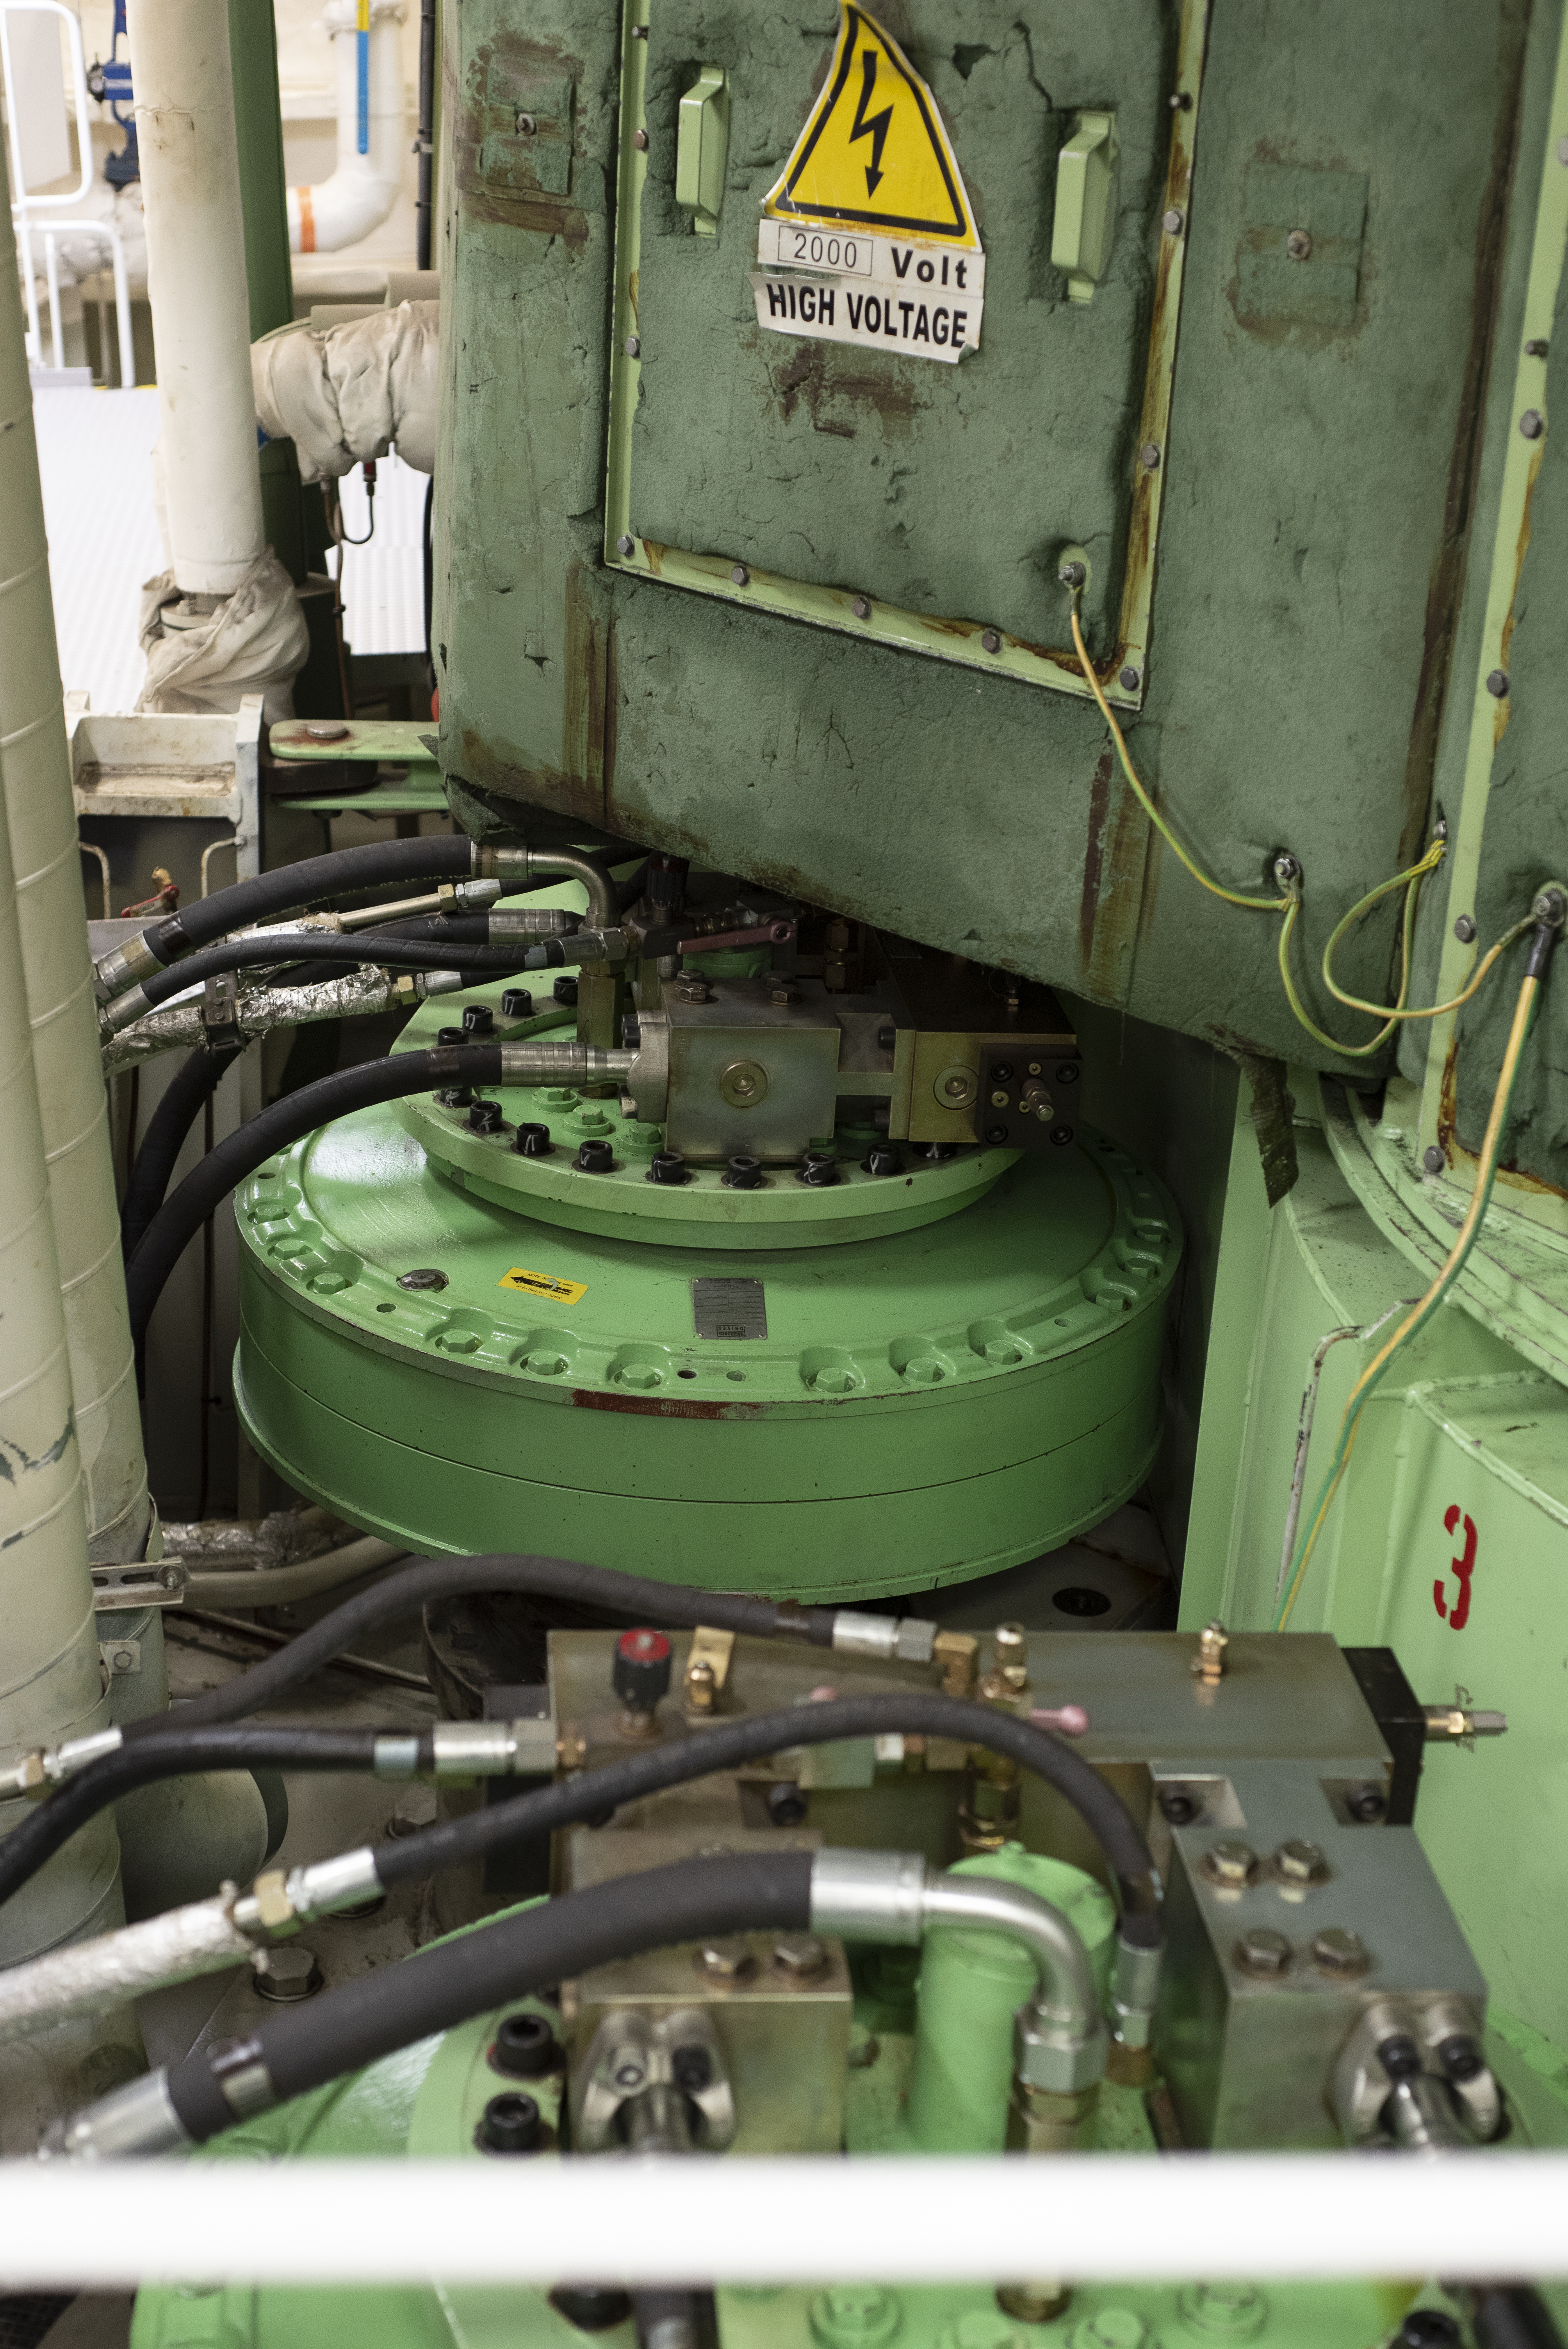
\includegraphics[width=10cm]{rotaryvane.jpg}\par
A rotary vane steering gear of an azimuth thruster aboard the MS Noordam
\end{center}

\subsection{Chain Steering Gear System}
In smaller vessels, a human element may be powerful enough for rudder rotation. A typical configuration for this system is the Chain, or Wire steering gear system. The wheel of the ship is connected directly to the rudder stock via a chain and azimuthing sprocket wheel. In this configuration, a pulling force is applied either clockwise or anticlockwise. This configuration is relatively cheap, and requires no electrical or hydraulic installations, and is therefore suitable for smaller yachts or personal vessels. Additionally, sheaves may be included for more torque, for performance sailboats.
\section{Cargo Handling}
\subsection{Cranes}
A crane is ascribed as any type of machine, generally equipped with a hoist rope, wire ropes or chains, and sheaves, that can be used both to lift and lower materials and to move them horizontally. They provide a mechanical advantage for the moving of heavy loads. At sea, nearly every ship has one form or another of cranes. They may be as simple as davits, for lifting and discharging a liferaft, or may be multiple hundreds of tonnes lifting for pipelaying or other heavy lifts. Depending on the application, these can be AC or DC motors, or AC motors driving hydraulics or pneumatics. Recent advancements in technology allow for the cranes to be PLC controlled, sometimes even wirelessly, similar to the HIAD design on shore, allowing crew to be down on the deck while maneuvering the crane.
\begin{center}
\includegraphics[width=12cm]{crane}\par
The \textit{Wei Li}, a crane ship
\end{center}
\subsection{Forklifts}
Some ships may have a fleet of internal forklifts for cargo handling. Typically these are all electric, i.e. battery powered.
\begin{center}
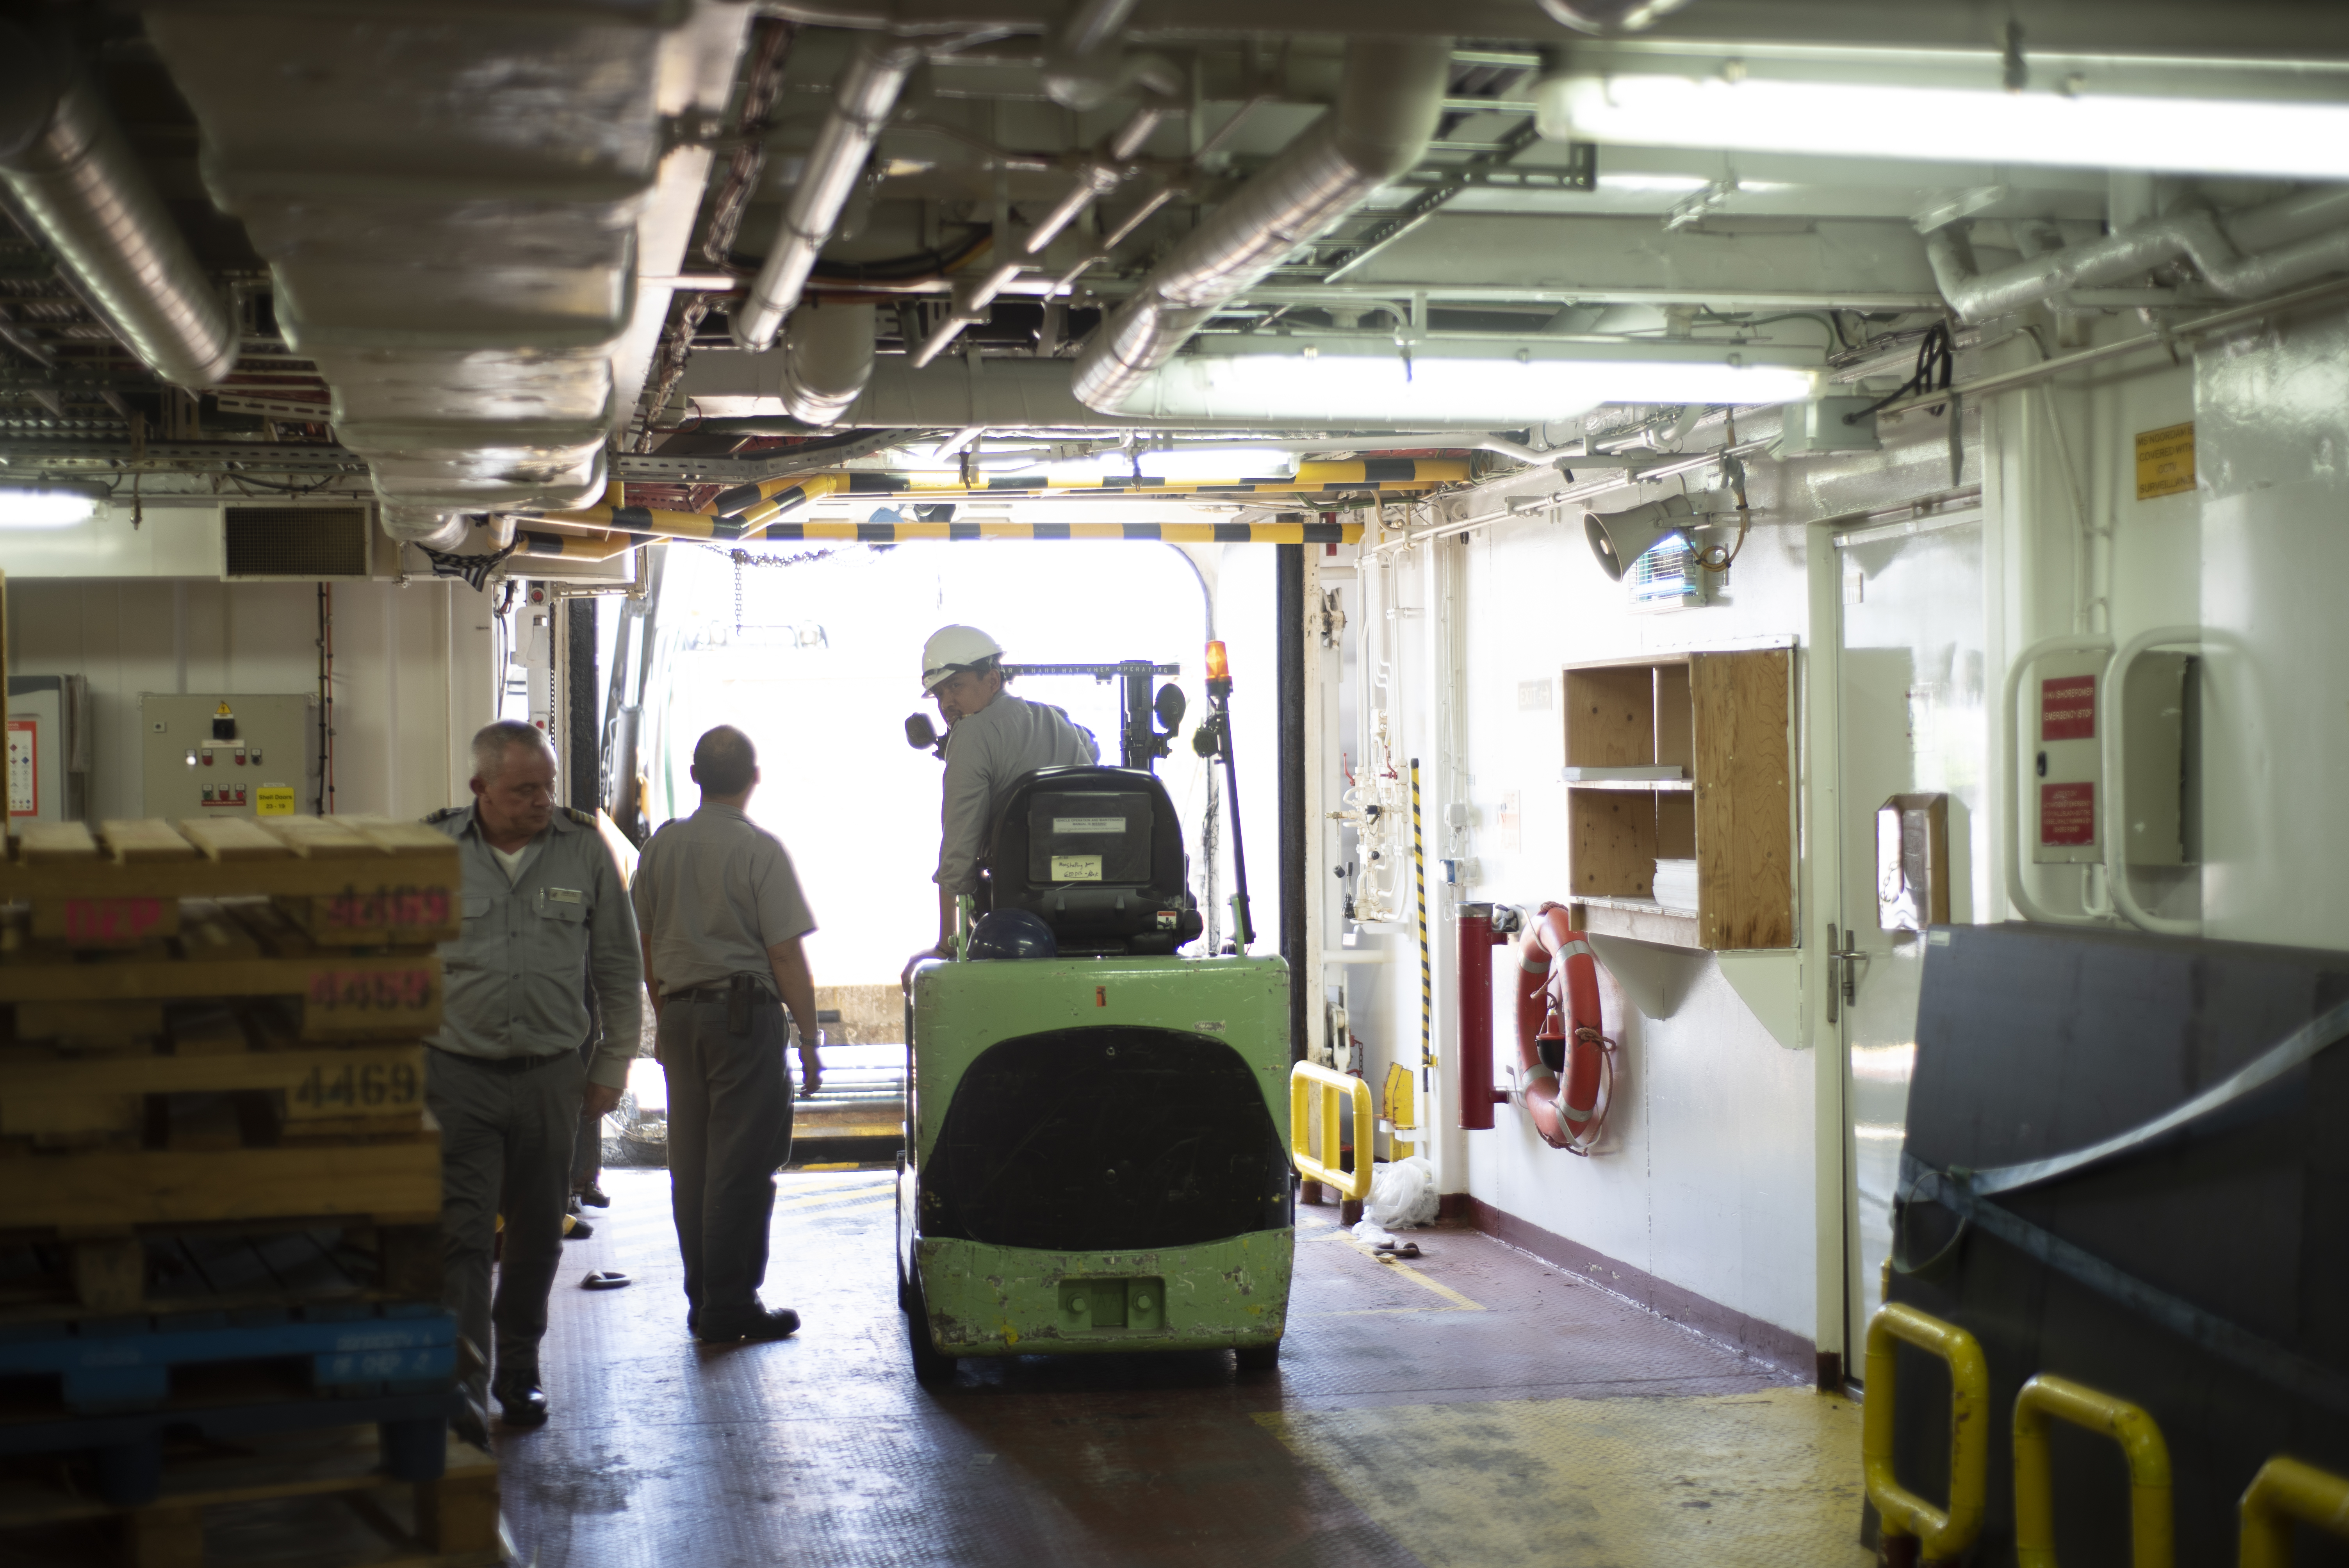
\includegraphics[width=12cm]{forklift}\par
The electric forklift aboard the MS Noordam
\end{center}
\subsection{Bulk Handling}
Bulk is any cargo which is solid but not secured in containers. This could be bulk ores, sugars, grains, etc. Handling bulk is very different to handling traditional cargo. Many ships will simply have multiple cargo holds to, the discharging and loading of cargo may be completely handled by the ports. Some bulk carriers may use an excavator on a traverse for the discharging of cargo, other bulk carriers may load the cargo on the ship as bulk but pack it in large bags for easy discharging. This is known as Bulk-In Bags-Out and is ideal for bulk carriers wishing to discharge to multiple ports along their voyage, as it decreases the machinery required at the ports, and reduces the workload if the bulk was to be bagged anyway.
\begin{center}
\includegraphics[width=12cm]{bulk}\par
The \textit{Sabrina I}, a bulk carrier, characterized by their flat cargo holds.
\end{center}
\subsection{Roll-On Roll-Off}
A type of vessel designed for taking upon wheeled cargo, such as cars, trucks, trailers or railroad cars, is the roll-on roll-off. This system allows for either a stern, bow or side ramp, or any combination of ramps, to load cargo by simply wheeling or driving it on, and vice-versa for discharing. These ramps are typically able to be lifted and stowed by use of hydraulic actuators, or very powerful electric motors, e.g. AC induction motors with a VFD for speed control. These ramps will also likely have limit switches to prevent being lowered too far, or raised in such a way to damage the ship.
\begin{center}
\includegraphics[width=12cm]{roro}\par
The \textit{Firmament Ace}, a car carrier.
\end{center}
\section{Hotel Systems}
Onboard ship there are is a plethora of equipment designed to improve the quality of life at sea. These are known as \textit{hotel systems}.
\subsection{Medical Services}
Medical Services include a defibrillator, which is powered by a battery bank with up to 300 uses, though, once used it is common for a defibrillator to be discarded and replaced. Some ships may also carry dive tanks and dive tank refilling services, including their own compressor.
\subsection{Galley Equipment}
Galley equipment includes everything related to the storage and preparation of food and foodstuffs at sea.
Ships will include refrigerators and freezers. These are driven off their own 3 phase AC induction compressor, and use a refrigerant in a closed refrigeration cycle. There are various temperatures used at sea, from $+12$ degrees $C$, down to $-40$ degrees $C$ for freezers. Depending on the size of ship, these may be walk-in and of extremely large size.

In addition, ships will have water purifiers. Ships will have fresh water tanks which first pass through reverse osmosis filtration plants. Depending on the requirement of the ship, these may be electrically assisted (i.e. AC induction pumps)

Depending on the size of the ship, they may also carry a desalination plant to remove salt and contaminants from sea water for use in drinking.

Some ships may also carry dumbwaiter systems for transporting food or laundry between decks. These are rated for between 5 and 300 KG, and may include additional features such as heating, cooling, or simply insulation. They are typically rated at an ascent and descent velocity of between 0.2 and 0.3 m/s. Specialized dumbwaiters for use on oil and gas industry ships are also designed to prevent electrostatic discharge and cable friction sparking. In many situations the dumbwaiters are driven by an AC induction motor attached to an automated variable speed drive for soft ascension and descension.

The majority, if not all, heating and cooking equipment in the galley is electrical using resistive heating.
\begin{center}
\includegraphics[width=8cm]{dumbwaiter}\par
A BKG service lift for foodstuffs
\end{center}
\subsection{Networks}
Internal and external communication is extremely important for life at sea. Both for safety \& security, as well as entertainment purposes.
\subsubsection{Internal}
Internal networks include any system where data is not incoming or outgoing directly to anywhere other than the ship, or does not require immediate delivery outside of the ship.
\subsubsection{Ship Communication}
\subsubsection{CCTV}
 Many companys will choose to install CCTV in their ships to deter theft, and to assist in the prosecution of any criminals when they return to shore. These cameras are wide angle of 14-20mm, and work either by low framerate constant recording, low framerate motion detection recording, high framerate motion detection recording or in "high risk" areas, some ships may opt for a high framerate constant recording. Framerates range from 3 to 30 fps, and cameras will include a very small internal memory of ~8 seconds to allow recovery of footage prior to their destruction, otherwise, footage will be transmitted wirelessly (on smaller vessels) or via the internal ethernet and stored in an area where usually only the captain, designated security officer, or potentially chief staff members may access.
\subsubsection{Intranet}
Many ships today will have intranet facilities available. On some ships, these may include training resources, ship internal communications (e.g. staff announcements or staff-to-staff private messaging). Additionally, the intranet systems will include access to any relevant resources about the ship, such as the ship's drawings, and the manufacturer's guides on any equipment, as well as an up-to-date copy of the IMDG, SOLAS, IMO codes etc, making it a valuable tool for staff.
\subsubsection{External}
External communication includes any system which requires an outside connection to either receive or transmit information.
\subsubsection{Internet}
Two kinds of internet exist on ships today. These are radio wireless local area networking of devices based on the IEEE 802.11 standards, commonly referred to as WiFi. These are delivered to staff and passengers alike by use of a satellite receiver. Cruise ships typically invest a huge amount of money on improving satellite connection speeds. In addition with certain techniques such as page caching and compression, internet for passengers will be quite fast, though it will never be as fast as a hardwired connection. Cruise ships may also charge an additional fee to their passengers for use of the internet, allowing the company to make a return on their investment.

The other kind of internet, though it is exclusively available on the latest cruise ships, are repeater towers. These either take a land-based 2, 3 or 4G signal and boost the frequency, allowing for calls-to-home to be made while close to shore, or by satellite assisted uptake receivers, allowing a regular shore-based cellphone signal to be transmitted via transducer and distributed to shore by use of a middle-man company, usually a large shore-based telecom. This system is unusual, however, and extremely expensive. Typically it is reserved for the cutting edge of cruise ship technology.
\subsection{Dynamic Positioning}
Dynamic Positioning, or DP, is an umbrella term for using enhanced sensory data, both internally (wind sensors, etc) and externally (GPS or DGPS, etc) to allow ships to automatically use their propulsion systems to remain at a single point, as close to stationary as possible. It should be noted that in its current form, DP is exclusively a \textit{reactive} system, and therefore will not always offer perfect results, as it has no way of predicting wind or ocean current changes.
\begin{center}
\includegraphics[width=10cm]{dp.jpg}\par
A DP system on a platform supply vessel, and what tools it uses to adjust for the various types of movement a ship may perform.
\end{center}
\subsection{Incinerator}
Incinerators onboard ships are used to incinerate sludge oil, food waste and other waste on ships. These products, under MARPOL, cannot be disposed of overboard. While they may be discharged at the next port of call, before doing so they often produce a terrible stench.

Incinerator is in the shape of a vertical cylindrical chamber with an inverted funnel shaped chimney at the the top. The cylindrical chamber consists of a burning chamber just as in case of oil fired burners, which are lined with refractory materials at the inside. An oil fired burner is provided to initiate the ignition process. It is extremely important that the temperature inside the cylinder is controlled and for this reason thermostats are used. To provide an uninterrupted flow of air for the combustion, forced draft fans are provided. The air supplied is directed upwards in swirls with the help of strategically designed ports.

A rotating shaft with blades is attached at the center, which helps for a faster combustion process and also prevents incomplete combustion. The ash and the residue thus generated due to the combustion is forced at the periphery by this rotating shaft. The ash is pushed into an ash hopper and it gets collected there. A door is provided to dump the waste inside the incinerator. This door pneumatically operated and when opened shuts down the fan and the burner automatically.

Not all the ash gets collected in the ash hopper. Some of the ash due to the forced air goes up to the chimney with the smoke. To remove this ash from the smoke a char eliminator is used. A char eliminator is similar to a filter paper. A sight glass is provided at the side of the incinerator to keep a watch at the burning process. All the processes are controlled with the help of a control panel that is fitted on or near the incinerator.

The latest advancements in incinerator technology from companies such as TeamTec and Hyundai offer additional levels of PLC-controlled temperature and discharge, meaning that maximum pollution levels can be raised or lowered depending on the regulations of the ruling state.
\subsection{Laundry Services}
Laundry will use a combination of three-phase washing machines, typically 440V, as well as steam from the ship's boilers. The operation of which is very similar to industrial applications on land, however the capacity is typically larger and the current drawn is typically lower due to the induction motor performing better on three phases. The capacity is typically 10 or 15 KG and, depending on the ship, there could be between 2 to 24 of them. As for steam, the advantage is removing any odours, as well as removing wrinkles without the need of ironing, and as it is simply air and water being used to clean, no chemicals are needed.
\subsection{Elevators}
Many ships carry elevators, especially passenger ships. These are for transporting occupants, or potentially goods on trolleyjacks between decks. These are fail-to-safe, meaning that they will not fall if a failure occurs, due to tensioned wires on either side of the elevator. These are usually powered by a three-phase AC induction motor with a VFD for speed control, however some ships may require additional lifting power for the transport of machinery or cargo and may opt for hydraulic actuators instead.
\newpage
\addcontentsline{toc}{section}{Learning Outcome 2}
\begin{tcolorbox}[colback=red!5!white,colframe=red!75!black,title=\textbf{Demonstrate basic knowledge of the operation of electro technical systems on board}]
\textit{Please reference document} \textbf{ETR Course 3 942.468} \textit{pages 2 and 3}
\end{tcolorbox}
\section{Glossary}
\subsection*{Current}
An \textbf{electric charge} is ascribed as either a \textit{positive} or \textit{negative}.\cite{e1} \textbf{Electric current} is defined as the movement, or \textit{flow} of electric charge past a point, or region.\cite{e3} An electric current is said to exist when there is a net flow of electric charge through a point.\cite{e4} In alternating current the motion of the electric charges is periodically reversed; in direct current it is not. Current is usually denoted by the symbol $I$.\cite{e5} The \textit{International System of Units} defines electric current as the $ampere$, symbol: $A$, which is the flow of electric charge across a surface at the rate of one coulomb per second.\cite{e2}
\subsection*{Voltage}
\textbf{Voltage, electric potential difference, electric pressure,  electric tension,} or \textbf{electromotive force} is the difference in electric potential between two points.\cite{e1} This is otherwise defined as the \textit{work} needed per unit of \textit{charge} to move a "test charge" between the two points.\cite{e4} Voltage is usually denoted by the symbol $\Delta V$ or $\Delta U$, or simply $V$ or $U$ for $Volts$, although it is sometimes referenced as $E$, or $emf$, i.e. \textbf{E}lectro\textbf{M}otive \textbf{F}orce. Like the Ampere, it is a \textit{International System of Units} "base unit"\cite{e2}
\subsection*{Impedance}
\textbf{Electrical impedance}, \textbf{complex impedance} or simply \textbf{impedance} is the opposition which components in a circuit, including the conductor, present to current when an electromotive force is applied.\cite{e6} Impedance is measured in \textit{Ohms} $\Omega$. There are three \textit{generalized} components of impedance. \textbf{Inductance}, which is exclusively present in \textit{alternating current} circuits. \textbf{Capacitance}, which is exclusively present in alternating current circuits. Finally, there is \textbf{resistive impedance}, or simply \textbf{resistance}, which acts identically in both \textit{direct current} and alternating current circuits.
\subsection*{Resistance}
\textbf{Resistive Impedance}, or simply \textbf{resistance} is a component of \textit{electrical impedance} and is defined as the third component to Ohm's Law. That is, where an electromotive force is applied, a current will flow. The opposition posed by the material in which an electron flow is present is ascribed as \textbf{resistance}. The \textit{International System of Units} defines Resistance as measured in \textit{Ohms}, $\Omega$. Resistance inhibits the flow of electrons identically to both direct current and alternating current circuits. That is, frequency $f$ has no effect on resistance. \textbf{Resistors} are common passive electrical components which intentionally implements resistive impedance.
\subsection*{Capacitance}
\textbf{Capacitance} is defined as the \textit{difference}, or ratio of change in \textit{electric charge}, against a corresponding change in \textit{electric potential}. Capacitance is divided into two categories: \textbf{self capacitance} and \textbf{mutual capacitance}. Capacitance is measured in $Farads$ $F$. However, in most electrical circuits, a $Farad$ is significantly larger than the capacitors used. Therefore, it is not uncommon to see MicroFarad ($\mu F$), NanoFarad ($nF$), or PicoFarad ($pF$) capacitors. It should also be noted that capacitance is an effect exclusively present on \textit{alternating current} circuits. In capacitors, a phenoma occurs whereby the current in the circuit lags behind the voltage, which generates \textit{reactive power}.
\subsection*{Self Capacitance}
Usually when discussing \textit{capacitance} it is usually referencing \textit{mutual} capacitance. However, for an \textbf{isolated} conductor there is a property of self-capacitance. Self-capacitance is the amount of electric charge that must be added to an isolated conductor in order to raise its electric potential by one volt.\cite{e7}
\subsection*{Mutual Capacitance}
The most commonly mentioned form of capacitance is \textit{mutual capacitance}. Mutual capacitance is where two conductors are separated by an insulating, or \textit{dieletric} material.
\subsection*{Inductance}
\textbf{Inductance}, or more accurately \textbf{self-inductance} is the property of an electromotive force being applied in opposition, i.e. opposing polarity, to the current in the inductive conductor. Any charge flowing through the circuit loses potential energy when transitioning from the higher voltage to the lower voltage section. Energy required to overcome the 'potential threshold' is stored in a magnetic field around the  inductive conductor. A current $i$ flowing through a conductor generates a magnetic field around the conductor, which is described by Ampere's circuital law. The total magnetic flux through a circuit $\Phi$ is equal to the product of the magnetic field and the area of the surface spanning the current path. If the current varies, the magnetic flux $\Phi$ through the circuit changes. By Faraday's law of induction, any change in flux through a circuit induces an electromotive force (EMF) or voltage $v$ in the circuit, proportional to the rate of change of flux. The unit for inductance is a $henry$ Symbol: $H$. An electrical circuit is ascribed the inductance of one henry when an electric current that is changing at one ampere per second results in an electromotive force of one volt across the inductor.
\subsection{Common Conversions \& Calculations}
\subsection{Ohm's Law Relationships}
Ohm's law states that the current through a conductor between two points is directly proportional to the voltage across the two points, and inversely proportional to the resistance presented in the circuit.\cite{e6}
Using this, we can show that

$I = \frac{V}{R}$

where $I$ is \textit{electric current}, measured in $Amps$,

$V$ is \textit{electromotive force}, or \textit{Voltage}, measured in $Volts$,

and $R$ is \textit{resistive impedance}, measured in \textit{Ohms} $(\Omega)$.

An example would be a voltage source of 12V with a circuit presenting a resistance of 40 Ohms:

\begin{center}
\includegraphics[width=5cm]{SimpleResistive.png}\par
\textit{* Assuming the conductor has no internal resistance}
\end{center}
In this circuit, we can calculate the current $I$ using Ohm's Law.

$I = \frac{V}{R}$ $\implies$ $I = \frac{12 V}{40 \Omega} = 0.3$ $\therefore$ $I = 0.3$ $Amps$

We can also use Ohm's Law to calculate the voltage, assuming we have the resistance and the current, or the resistance, assuming we have the voltage and current.
\subsection{Joule's First Law}
Joule's first law, also known as the Joule–Lenz law, states that the power of heating generated by an electrical conductor is proportional to the product of its resistance and the square of the current:

$P \propto I^2 R$

Furthermore, in direct current circuitry, we can also calculate $P$ using the formula:

$P = V I = I^2 R = \frac{V^2}{R}$

Using the same circuit as before, we can calculate the resistor of $40 \Omega$ will produce a heating effect as losses as:

$P = \frac{V^2}{R}$ $\implies$ $P = \frac{12V^2}{40 \Omega} = 3.6$ $\therefore$ $P = 3.6$ $Watts$

\subsection{Impedance}
Impedance $Z$, measured in Ohms ($\Omega$) in direct current circuits is exclusively the resistive opposition to current. In alternating current ciruits, it is the sum reactance ($X$) of \textit{resistive impedance}, \textit{capactive reactance} and \textit{inductive reactance}. To calculate the total impedance of a circuit, it is necessary to use multiple formula to first establish the capacitive reactance and inductive reactance components of the circuit. We can do this using the formulas:

$X_C = \frac{1}{2\pi fC}$

Where $X_C$ is the capacitive reactance, $f$ is the frequency of the AC supply, and $C$ is the capacitance, measured in $Farads$

\textit{and}

$X_L = 2\pi fL$

Where $X_L$ is the inductive reactance, $f$ is the frequency of the AC supply, and $L$ is the inductance, measured in $Henries$

Impedance, $Z$ can be calculated using Pythagoras' Theorem, as the phasors presented here produce a right-angled triangle, commonly referred to as the "impedance triangle" which can be represented as such:

\begin{center}
\includegraphics[width=8cm]{Impedance.png}
\end{center}

Therefore, the Pythagoras' formula for finding the hypoteneuse of a right-angle triangle:

$a^2 + b^2 = c^2$

can be used to calculate the impedance, $Z$. Here is an example of a "RLC" circuit, which contains a \textbf{R}esistor, Inductor (\textbf{L}) and a \textbf{C}apacitor.

\begin{center}
\includegraphics[width=12cm]{RLC.png}\par
\textit{* Assuming the conductor has no internal impedance}
\end{center}
Calculate the reactance of the capacitor:

$X_C = \frac{1}{2\pi fC}$ $\implies$ $X_C = \frac{1}{2\times \pi \times 50 \times (12.5 \times 10^{-6})} = 254.64791$ $\therefore$ $X_C \approx 254.7 \Omega$

Calculate the reactance of the inductor:

$X_L = 2\pi fL$ $\implies$ $X_L = 2 \times \pi \times 50 \times 0.6 = 188.49556$ $\therefore$ $X_L \approx 188.5 \Omega$

Calculate the total impedance:

$Z = \sqrt{{X_R}^2 + (X_L - X_C)^2}$ $\implies$ $Z = \sqrt{95^2 + (188.5 - 254.7)^2} = 115.79050$ $\therefore$

$Z = 115.79 \Omega$
\subsection{Resistors in Parallel vs. Series}
As previously mentioned, resistors behave identically in both AC and DC circuits -- that is, limiting the flow of current by a certain amount. These are passive components with no moving parts, simply a unique material which slows any current flow. As a disadvantage, however, resistors generate heat as a byproduct as per Joule's First Law. Furthermore, they also behave differently when placed in series than when they are placed in parallel. When in series, the current is the same for all elements.

$I = I_1 = I_2 = \ldots = I_n$

And the voltage is not common to each component, however the total voltage is the sum of voltage drops of the individual components.

$V = V_1 + V_2 + \ldots + V_n$

For instance:

\begin{center}
\includegraphics[width=10cm]{Resistor1.png}\par
\textit{* Assuming the conductor has no internal resistance}
\end{center}
We can use Ohm's Law to calculate the current of this circuit:

$I = \frac{V}{R}$ $\implies$ $I = \frac{12V}{(25\Omega + 10\Omega + 50\Omega)} = 0.14117647$ $\therefore$ $I \approx 0.14$ $Amps$

We can also prove Kirchoff's Voltage Law which purports that the directed sum of the potential differences (voltages) around any closed loop is zero. To do this, we need to calculate the voltage drop across each resistor. We use Ohm's Law once again to calculate this for each instance:

$V = I \times R$ $\implies$

$V_1 = 0.14 \times 25 = 3.5$ $Volts$

$V_2 = 0.14 \times 10 = 1.4$ $Volts$

$V_3 = 0.14 \times 50 = 7$ $Volts$

$V_1 + V_2 + V_3 \overset{!}{=} V$ $\therefore$ $3.5V + 1.4V + 7V + -12V \approx 0$

And we can see that for this circuit Kirchoff's Voltage Law is proven to be true.

In parallel, however, the voltage is common to each component:

$V = V_1 = V_2 = \ldots = V_n$

To find $I_{total}$ we need to use Ohm's Law formula:

$I_{total} = V(\frac{1}{R_1} + \frac{1}{R_2} + \ldots + \frac{1}{R_n})$

And to find the total resistance, we can add the reciprocals of the resistances $R_i$ and take the reciprocal of the sum:
$\frac{1}{R_{total}} = \frac{1}{R_1} + \frac{1}{R_2} + \ldots + \frac{1}{R_n}$

For instance, in this circuit:

\begin{center}
\includegraphics[width=10cm]{Resistor2.png}\par
\textit{* Assuming the conductor has no internal resistance}
\end{center}


We can find the total resistance $R_{total}$

$\frac{1}{R_{total}} = \frac{1}{R_1} + \frac{1}{R_2} + \ldots + \frac{1}{R_n}$ $\implies$ $\frac{1}{R_{total}} = \frac{1}{25 \Omega} + \frac{1}{10 \Omega} + \frac{1}{50 \Omega} = 0.16$

$\therefore$ $R_{total} = \frac{1}{0.16} = 6.25$ $\Omega$

Furthermore, we can find the total current of the circuit using the calculation:

$I = \frac{V}{R}$ $\implies$ $I = \frac{12V}{6.25 \Omega} = 1.92$ $\therefore$ $I = 1.92$ $Amps$

or

$I_{total} = V(\frac{1}{R_1} + \frac{1}{R_2} + \ldots + \frac{1}{R_n})$ $\implies$ $I = 12V\times (\frac{1}{25\Omega} + \frac{1}{10\Omega} + \frac{1}{50\Omega}) = 1.92$

And we can calculate the current drop over each component using the following formula:

$I = \frac{V}{R_i}$ $\implies$ $I_1 = \frac{12}{25} = 0.48$ $Amps$

$I_2 = \frac{12}{10} = 1.2$ $Amps$

$I_3 = \frac{12}{50} = 0.24$ $Amps$

$I_{total} \overset{!}{=} I_1 + I_2 + I_3$ $\therefore$ $0.48+1.2+0.24 = 1.92$
\subsection{Energy}
Energy is ascribed as $Power \times Time$. For instance, Watts multiplied by time can be ascribed as Watt-hours.
\subsection{Metric Prefixes}
When dealing with units of various sizes, it may be beneficial to understand the prefixes of the metric measurement system in order to determine the true value of any given unit. Here is a simplified table of the prefixes:
\begin{center}
\begin{tabular}{| l | l | l |}
  \hline
Prefix Name & Symbol & Base 10 \\
  \hline
yotta & Y & $10^{24}$ \\
  zetta & Z & $10^{21}$ \\
  exa & E & $10^{18}$ \\
peta & P & $10^{15}$ \\
tera & T & $10^{12}$ \\
giga & G & $10^9$ \\
mega & M & $10^6$ \\
kilo & k & $10^3$ \\
hecto & h & $10^2$ \\
deca & da & $10^1$ \\
- & - & $10^0$ \\
deci & d & $10^{-1}$ \\
centi & c & $10^{-2}$ \\
milli & m & $10^{-3}$ \\
micro & $\mu$ & $10^{-6}$ \\
nano & n & $10^{-9}$ \\
pico & p & $10^{-12}$ \\
femto & f & $10^{-15}$ \\
atto & a & $10^{-18}$ \\
zepto & z & $10^{-21}$ \\
yocto & y & $10^{-24}$ \\
  \hline
\end{tabular}
\end{center}

For instance: A MicroFarad is expressed as $\mu F$ and represents a value of $10^{-6}$. Therefore $50 \mu F$ would be equivalent to $0.00005$ Farads
\subsection{AC vs DC}
The primary difference between \textbf{alternating current} and \textbf{direct current} is the method of transmission of electrical charge. Direct Current has a \textit{positive} and \textit{negative} point. By convention, the direction of current flow is from the positive terminal to the negative terminal, although in reality the electron flow is opposite.\cite{e6} Alternating Current, on the other hand, has one or more \textit{phases}. In shore-based applications, generally this is a single phase, with the other terminal providing a neutral, or ground, providing an electric potential, allowing current flow. These live phases have a rotating waveform known as a \textit{sinusoid}. A period of positive electron flow is then followed by a period of negative electron flow. The length of the total period is measured in $Hertz$ ($Hz$). While this frequency may be theoretically any number from $>0 Hz$ upwards, tending towards $\infty$. It should be noted, however for calculation purposes that direct current has a frequency of $0$, and this lack of frequency is why there is no capacitance or inductance component in direct current circuits.
\subsection{R.M.S.}
\textbf{R.M.S.}, \textbf{root-mean squared}, or \textbf{quadratic mean} is shorthand for the square of the function that defines the continuous waveform, typically of an AC supply. For a sine wave, the R.M.S. is exactly 0.707 of the peak-to-peak voltage. The R.M.S. value is important as it represents the direct-current equivalent, i.e. visible output in electronics. For instance:

\begin{center}
\includegraphics[width=6cm]{RMS.png}\par
\textit{* Assuming the conductor has no internal resistance}
\end{center}

Using the equation $P = I^2 \times R$ we can calculate the wattage output of the resistor on direct current or alternating current.

On DC: $P=\frac{V^2}{R}$ $\implies$ $P = \frac{100^2V}{120\Omega}=83.33\circ Watts$

The peak-to-peak voltage of 100V R.M.S. AC is, however:

$V_{peak} = V_{r.m.s} \times \sqrt{2} = 141.42136 V$

If we were to take a peak-to-peak value of 100V for this calculation, the wattage we would create would be:

$P=\frac{V_{peak}^2}{R}$ $\implies$ $P = \frac{70.7V^2}{120\Omega}\approx 41.65$ $Watts$
\section{Electromagnetic Induction}
Influence of Magnetic Field on Conductor
describes principles of self and mutual induction as well as self and mutually induced e.m.f
compares coil inductance with and without iron core
\subsection{Fleming's Rule}
Fleming's Rule to determine directions of magnetic field, motion and Current
When there is a current carrying conductor is acted upon by a magnetic flux, as per Faraday's Law, a force will also act upon the conductor. The direction of this force can be found using Fleming's "Left Hand Rule", which is sometimes referred to as Fleming's Left Hand Rule for Motors". This force is found to be perpendicular to both the directions of current and of magnetic field.
\begin{center}
\includegraphics[width=6cm]{flem2.png}
\end{center}
While current flows through a conductor, one magnetic field is induced around it. The magnetic field can be imagined by considering numbers of closed magnetic lines of force around the conductor. The direction of magnetic lines of force can be determined by Maxwell’s corkscrew rule or right-hand grip rule. As per these rules, the direction of the magnetic lines of force (or flux lines) is clockwise if the current is flowing away from the viewer, that is if the direction of current through the conductor is inward from the reference plane as shown in the figure.\cite{e8}
\begin{center}
\includegraphics[width=6cm]{flem.jpg}
\end{center}

Fleming's Right Hand Rule proves to be equal and opposite, sometimes known as "Fleming's Right Hand Rule for Generators". Whenever a conductor moves inside a magnetic field, there will be an induced current in it. If this conductor gets forcefully moved inside the magnetic field, there will be a relation between the direction of applied force, magnetic field and the current.
\begin{center}
\includegraphics[width=6cm]{fleming-right-hand-rule.jpg}
\end{center}
\subsection{Faraday's Law}
\epigraph{The electromotive force around a closed path is equal to the negative of the time rate of change of the magnetic flux enclosed by the path.}{\textit{Michael Faraday}}
Faraday’s Law of Electromagnetic Induction describes how an electric current produces a magnetic field and, conversely, how a changing magnetic field generates an electric current in a conductor.\cite{e9}\cite{e5}

Faraday visualized a magnetic field as composed of many lines of induction, along which a small magnetic compass would point. The aggregate of the lines intersecting a given area is called the magnetic flux. The electrical effects were thus attributed by Faraday to a changing magnetic flux. Some years later the Scottish physicist James Clerk Maxwell proposed that the fundamental effect of changing magnetic flux was the production of an electric field, not only in a conductor (where it could drive an electric charge) but also in space even in the absence of electric charges. Maxwell formulated the mathematical expression relating the change in magnetic flux to the induced electromotive force (E, or emf). This relationship, known as Faraday’s law of induction (to distinguish it from his laws of electrolysis), states that the magnitude of the emf induced in a circuit is proportional to the rate of change of the magnetic flux that cuts across the circuit. If the rate of change of magnetic flux is expressed in units of webers per second, the induced emf has units of volts. \cite{e5}
\subsection{Lenz's Law}
\epigraph{Nature abhors a change in flux.}{\textit{D.J. Griffiths}}
Lenz's law states that when an emf is generated by a change in magnetic flux according to Faraday's Law, the polarity of the induced emf is such, that it produces an current that's magnetic field opposes the change which produces it. Thrusting a pole of a permanent bar magnet through a coil of wire, for example, induces an electric current in the coil; the current in turn sets up a magnetic field around the coil, making it a magnet. Lenz’s law indicates the direction of the induced current. Because like magnetic poles repel each other, Lenz’s law states that when the north pole of the bar magnet is approaching the coil, the induced current flows in such a way as to make the side of the coil nearest the pole of the bar magnet itself a north pole to oppose the approaching bar magnet. Upon withdrawing the bar magnet from the coil, the induced current reverses itself, and the near side of the coil becomes a south pole to produce an attracting force on the receding bar magnet.\cite{e5}
\section{Fundamentals of Electrical Machines}
Generally speaking, an electrical machine is ascribed as any machines using electromagnetic forces, such as electric motors, electric generators, and others. They convert electric forces into mechanical forces, or mechanical forces into electrical forces. Transformers are also included as a type of electrical machine. All electrical machines require a conductor, and therefore, in addition to taking advantage of the tensile strength of steel, copper is used for its effectiveness as a conductor and low cost. However, theoretically any motor or generator could use any conductive material.
\subsection{AC Electrical Machines}
Electrical machines relying on alternating current to perform most of the \textit{work} fall into two classifications. Both rely heavily on magnetic forces and electromagnetic induction, as described by Faraday's and Lenz's Laws. These machines are able to function as either a generator or motor, depending on the configuration. That is to say, the action by which electric energy is converted to mechanical energy, and vice-versa, is reversible when dealing with AC electrical machines. These machines are ideal for medium to high power applications, especially when used in tandem with hydraulic machines or diesel engines, giving them incredible power output and relatively cheap, reliable construction. In all AC electrical machines, it is preferable to use laminated steel on their stator core, to reduce the effect of eddy currents, which are loops of electrical current induced within conductors, running perpendicular to the plane of the flux.
\subsection{AC Generators}
\textbf{Synchronous generators}, which use an \textit{AVR}, an Automatic Voltage Regulator, providing DC excitation inverted to AC, producing an electromagnetic effect on the rotor, or, alternatively, they may use an arrangment of permanent magnets.
\begin{center}
\includegraphics[width=10cm]{sync.jpg}
\end{center}
These are the most common form of generator aboard ships, as they reliably produce a given frequency, and are able to do so without a pre-existing line voltage. However, they require synchronization to work in parallel. It is important to maintain a consistent RPM with synchronous generators, in order to provide useful power to the network. The number of projected poles determines the relationship between the RPM and the frequency produced. The relationship between the frequency produced can be expressed as follows:

$f=\frac{N\times p}{120}$

where $f$ is the frequency produced, $N$ is the RPM of the generator's rotor, $p$ is the number of poles, and 120 is required to de-couple $N$ from the time factor of 60 seconds, multiplied by 2 for each half of the sine-wave produced. Typically, a 14-pole 514 RPM, 60 Hz arrangement is used for primary generation on ships. Emergency, shaft, or turbo generators may have different configurations.

\textbf{Induction generators} operate by mechanically turning their rotor faster than the synchronous speed, giving negative slip. A regular AC asynchronous motor usually can be used as a generator, without any internal modifications. Induction generators are useful in applications such as minihydro power plants, wind turbines, or in reducing high-pressure gas streams to lower pressure, because they can recover energy with relatively simple controls. They do not require an exciter circuit because the rotating magnetic field is provided by induction from the stator circuit. They also do not require speed governor equipment as they inherently operate at the connected grid frequency.

To operate, an induction generator must be excited with a leading voltage; this is usually done by connection to an electrical grid, or sometimes they are self-excited by using phase correcting capacitors.
\subsection{AC Motors}
\textbf{Synchronous} motors rotate at the exact speed of the changing magnetic flux produced by the stator, and therefore their speed is indexed to the supply frequency. These motors require excitation on their rotor, or a permanent magnet arragement. This excitation may be by rectified DC brushes and slip rings, or it may be by a bridge rectifier located on the rotor itself. In high power applications, synchronous motors are highly efficient. However, construction is complicated, and typically a separate transformer is used for rectification. Azimuth thrusters by ABB and Rolls Royce utilize synchronous motors in their high power applications. Their slow RPM offsets the maintenance requirement of the DC brushes.

\textbf{Asynchronous} motors rotate slightly slower than the speed of the changing magnetic flux, in order to provide a relative difference, which generates an electromagnet effect on the short-circuited squirrel cage rotor. These machines are able to operate on single-phase. However, typically they perform significantly more efficiently and effectively on three-phase (or greater) power.

\begin{center}
\includegraphics[width=12cm]{asyncmotor.jpg}
\end{center}

There is no \textit{physical} connection required between the rotor (rotating) and stator (stationary) parts of an asynchronous AC motor, however, a bearing arrangement is necessary to maintain the relative position of the rotor to the stator. This is a significant advantage of AC motors over synchronous or DC motors. There is no need for a complex and maintenance-heavy brush and slip ring arrangement.

describes methods of AC motors start-up and speed control
given a motor name plate, explains the meaning of all the information displayed
\subsection{DC Electrical Machines}
\subsection{DC Generators}
DC Generators function on the principle of Faraday's Law of Induction. That is, when there is relative movement between a conductor and a magnetic force (or electromagnet), an electromotive force is induced in the conductor. A DC generator has six primary parts to its construction:
\begin{itemize}
\item Yoke

This is the outer frame of the generator. This is usually either cast iron, or steel. This provides mechanical strength to the generator, as well as carrying the magnetic flux produced by the field winding.
\item Poles / Pole Shoes

Poles are attached to the yoke. They carry the field winding and pole shoes are attached to them. Pole shoes serve two functions: supporting the field coils, and evenly spreading out the flux in the empty spaces of the generator.
\item Field Winding

These are the conductive material upon which the e.m.f. is induced upon. They are placed on each pole and connected in series. Particular attention is paid to their arrangement that, when energized, they form opposing North and South poles.
\item Armature core

This is the rotating center of the DC generator. It has slots to carry the armature windings, and is constructed of laminated steel to prevent eddy current losses. It has a key for connection to a shaft, and may additionally have ducting for axial air flow and cooling.
\item Armature Winding

This is the conductive material which is wound around the armature core's slots, which produces an e.m.f. when there is relative moment against the magnetic poles of the field winding.
\item Commutator / Brushes

In a DC generator, the function of the commutator and brush arrangement is to collect the e.m.f. from the armature and pass it on to be used as useful power.

\textit{It should be noted that in DC generators, the field windings may be replaced by permanent magnets. Recent advancements in magnetic construction (i.e. Neodymium) allows for a generator of reasonable size to be used. However, the maximum output of the generator $P_{out}$ is still limited by the strength over the magnets used.}
\end{itemize}
DC Generators fall into two categories: separately excited, and self-excited. Separately excited DC generators have their field windings energized by an external DC source. Self-excited DC generators have their field windings excited by the generator itself. The initial e.m.f. generation is due to the residual magnetism in the field poles. Self-excited DC generators can further be divided into three types: (a) Series wound - field winding in series with armature winding (b) Shunt wound - field winding in parallel with armature winding (c) Compound wound - combination of series and shunt winding.

DC Generators, due to the high maintenance requirement and complicated construction of the commutator and brush array are infrequently used in practical applications. They are, however, most commonly found as a portable generator, especially one which is required to output an unusual frequency, such as a portable generator to output 50Hz or 60Hz. In addition, a DC generator may also be used when there is a requirement for a range of voltages. Self-excited DC generators are inherently safe from short-circuits, as any short circuit will prevent the total current across the field to be 0, thereby de-exciting the generator.
\subsection{DC Motors}
DC Motors work on an identical principle as the DC generator, except the process is reversed. Both the field windings and the armature windings are energized, which produces useful mechanical power. Similar to Generators, recent advancements have been made in magnet technology, allowing a permanent magnet arrangement construction. Unlike the DC generator, however, the armature is stationary, and energized externally without the use of commutators and brushes. Permanent magnets are placed in the yoke, and the yoke is now free to rotate. This design is known as the brushless DC motor.

\begin{center}
\includegraphics[width=10cm]{bldc.jpg}\par
The Yoke of a Brushless DC Motor
\end{center}

DC motors have some advantages over their AC counterparts. DC motors are able to operate at any speed. Brushless DC motors also have simple, reliable construction, and with low maintenance requirements they are ideal for low to medium power requirements where variable speed is required. Examples of this in practical applications include Rolls Royce azimuthing thrusters, which have variable speed. These use a brush and commutator arrangement, however, their RPM is reasonably low, and maintenance on their brushes is minimal. Other applications include handheld power tools, such as drills or grinders, where variable speed may be required.
\section{Transformers}
Onboard ships, two kinds of transformers (with regards to phase) are present. Single phase transformers, and three phase transformers. These are subdivided into low and high voltages. The operation of a single phase transformer is quite simple. An electromotive force is applied to the primary winding, which generates an electromagnetic flux within a laminated steel core. This magnetic flux, as according to Faraday's Law of Electromagnetic Induction, induces an electromotive force in the secondary winding. This method is extremely power efficient, with power throughput ratios approaching 1:1. However, there is a small amount of impedance present in both windings, though this is negligible (<150 $\Omega$ typically, with some $P=I^2\times R$ losses).

Transformers are usually rated in apparent power (VA or kVA). Smaller transformers are generally air cooled, though some transformers demand oil cooling.

\begin{center}
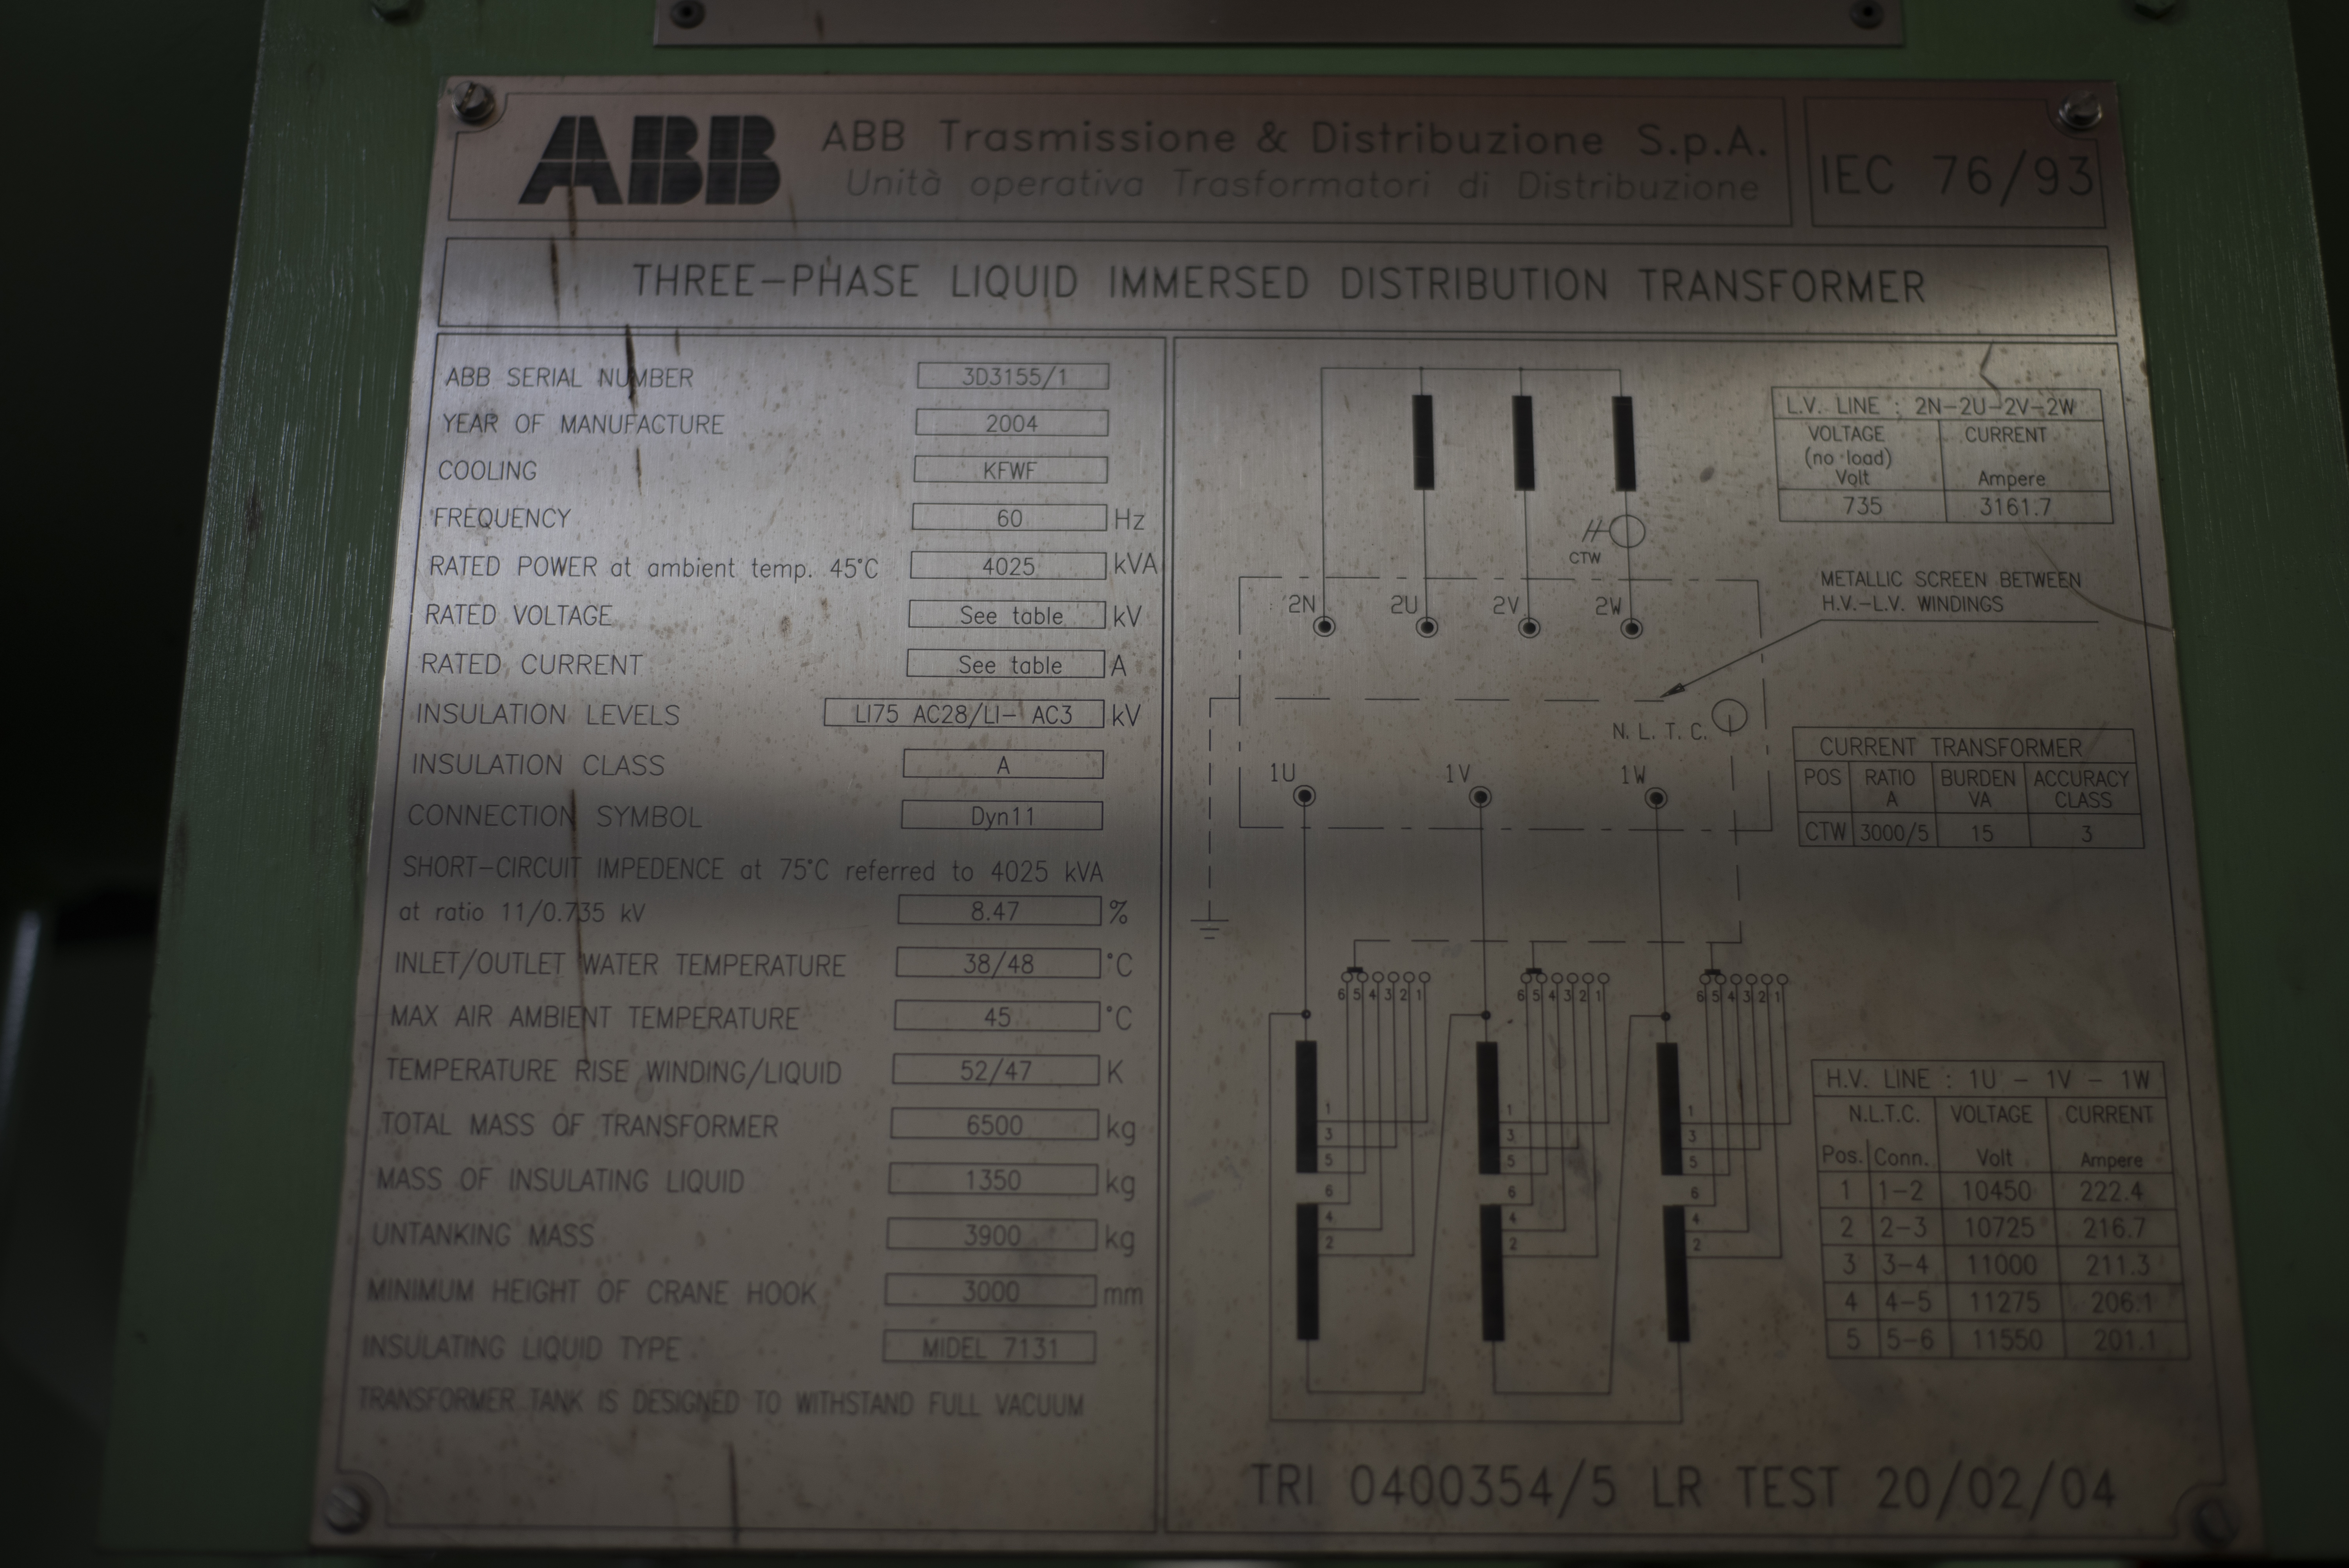
\includegraphics[width=12cm]{3phtrans.jpg}\par
The datasheet of a 11kV transformer aboard the MS Noordam
\end{center}

Three-phase transformers operate on a similar principle to single phase transformers. These contain three primary windings, and three secondary windings. Power transformers (i.e. high voltage, or high current throughputs) are typically connected in the Delta-Delta ($\Delta - \Delta$) arrangement. Three phase transformers also have an advantage in that if a fault occurs on a single phase, the faulty phase can be disconnected. This is known as Open-Delta or "V" connection. A three phase supply will still be available, albeit at a reduced current throughput.

Transformers are typically low maintenance, as they are solid-state. However, they should be checked regularly to ensure effective operation. Nearly all ships above a certain size will have some form of transformer, as typically a ship will generate at 440V AC or above, and will still require power for 240V consumers, or for delicate circuitry such as control circuits, 24V, 12V or even 5V. Transformers are used to accomplish this on AC.\cite[p. 29]{e11}

\begin{center}
\includegraphics[width=10cm]{transformertiny.jpg}\par
A 12V to 5.5V transformer
\end{center}

On DC, it should be noted that there are DC to DC converters for low-voltage applications. These are the Buck and Boost DC-to-DC Converters, which use a capacitor in parallel to effectively double the voltage and half the current. However, for power electronics, it is generally more effective to simply invert DC to AC and rectify AC to DC with a full bridge rectifier, for voltages higher than 24V.

\section{Electrical Distribution}
The primary function of an electrical distribution system is to safely deliver useful power to consumers aboard the ship. This is done by a prime generation machine -- usually a diesel generator -- and subdividing the resulting power via switchboards. These switchboards include rigorous safety systems. Most common of which is a circuit breaker -- a simple device which disconnects incoming power when it registers a current greater than which it is rated for. Typically, in addition to this circuit breaker, many systems will also include a thermistor, which will disconnect if a certain temperature -- generally indicating an overheating of wiring -- is detected. Typically ships will also be a three-phase insulated system. This system allows for a redundancy in which if a single phase has an earth fault, normal operation of the consumer will continue. High voltage ships will, however, be earthed resistively.

The standard circuit breaker for power electronics is the MCCB, a Moulded Case Circuit Breaker, which are generally rated for 50 to 1500 Amps. These include adjustable thermal overcurrent settings and an adjustable or fixed magnetic overcurrent trip for short circuit protection, and may even include an undervoltage trip coil. In addition, hundreds of MCBs (Miniature Circuit Breaker) are located on the ship. These are rated for 5-100 Amps, and typically include thermal overcurrent and magnetic short circuit protection.

In addition to the primary generators, there may be secondary or ancillary generators, but there will always be an emergency generator as required under SOLAS. This generator will have its own switchboard, from which all essential consumers are fed. These typically include any emegency lighting, fire pumps, one of the steering gears, an air compressor, etc. Recent ships may include an emergency generator capable of supplying AC or galley equipment as well, though this is not required.\cite[p. 19]{e11}

\section{Automation}
Automation in practical applications falls into two categories: low-level and high-level. Typically, low-level applications include PLCs of various functionality, or CAN bus controllers. Even simpler may be mechanical or electrical switches, such as pressure switch circuits. High-level applications include SCADA (Supervisory Control And Data Acquisition), or ethernet NAS (Network Attached Storage) controllers.

Automation is defined as the process or procedure by which an action may be performed without human assistance or intervention. The simplest examples of shipboard automation include tasks such as a circuit breaker tripping when too much current passes through it. A complex example includes PID (Proportional Integral Derivative) controller feeding real-time accurate information over ethernet to a microprocessor, gradually increasing or decreasing rotational velocity of a forced draft fan for cooling.

Automation requires three important aspects: information, logic, and instruction. These aspects may be contained within a single system. This is known as a closed loop feedback system. Information may be a boolean value, i.e. information with a value of either 0 or 1, or it may be numeric, e.g. a temperature, or alpha-numeric, e.g. a color or complex number. Logic is the decider. In simpler systems, these are often referred to as \textit{gates}. A logic gate may be a \textit{decider}, a \textit{comparator}, a \textit{constant} or an \textit{arithmetical} gate. Deciders take a single value (or the sum of multiple values) and compare it against a predetermined value. A simple example of a decider would be:

\textit{if} \textbf{temperature} $>$ $n$ degrees, \textit{then} \textbf{output}

Comparators take two or more signals (or two or more sums of signals) and outputs a numeric value, typically a boolean value. A simple example of a comparator would be:

\textit{if} \textbf{pressure one} $=$ \textbf{pressure two}, \textit{then} \textbf{output}

Arithmetic logic gates are intermediate gates designed to perform mathematical operations on incoming signals. These are less common, but very important when converting values. A simple example of an arithmetic gate would be:

\textbf{signal one} metres $\times$ 3.28084, \textbf{output} feet

Constant logic gates output a set of predetermined values. These may be boolean, numeric or alpha-numeric. Constant logic gates are used primarily to store a series of instructions, or to output multiple instructions which comparators may use in place of several decider gates. A simple example of a constant gate would be:

\textbf{output one}, \textbf{output two}, \textbf{output three}

Common logic gates include the \textbf{OR} gate, \textbf{AND} gate, \textbf{XOR} gate, \textbf{NOT} gate \textbf{XNOR}, and the \textbf{NAND} gate.

\textbf{OR} gates output a boolean value of 1 when either inputs are $>0$

\textbf{AND} gates output a boolean value of 1 when both (or all) inputs are $>0$.

\textbf{XOR} gates output a boolean value of 1 when one of the inputs is $>0$, but not both.

\textbf{NOT} gates output a boolean value of 1 when the single input is $>0$.

\textbf{NAND} gates output a boolean value of 1 when one of the following conditions are met: (a) both inputs are 0, (b) input one is $>0$, (c) input two is $>0$. Therefore, these are gates which are only disabled when both inputs are $>0$.

\textbf{XNOR} gates output a boolean value of 1 when one of the following conditions are met: (a) both inputs are 0, (b) both inputs are $>0$. Therefore, these gates are disabled when one of the two inputs is $>0$.

\begin{center}
\includegraphics[width=\textwidth]{gates.png}
\end{center}

PLCs, or \textit{Programmable Logic Controllers} make liberal use of logic gates, which they frequently refer to as \textit{Function Blocks}. In certain PLC systems, \textit{ladder} logic, or structured imperative languages. PLCs are very common in industrial applications for their simplified, robust designs. Typically, PLCs have two different kinds of inputs, these are digital (binary/boolean) inputs, and analogue (numeric/PID) inputs. PLCs typically also have several outputs. Usually these are simply digital, as analogue output is somewhat rare, though not unheard of, especially in expensive, high-end PLC systems. Additionally, PLC systems commonly have internal clocks for day/night control. In industrial applications, PLCs often control the coils of switches. A common application is in pressure switches. A PLC may control a dozen pressure switches of different tanks, enabling or disabling various pumps to ensure pressure falls within a specific range. The advantage of PLCs over more simplified control circuitry is the ability to enable at a bottom, or floor value, and disable at a top, or ceiling value. PLC software is often used to alter these values manually, or even automatically based on other factors. An example of this would be to maintain the pressure of a tank, but also measuring atmospheric temperature to account for temperature-based expansion and condensing.

\begin{center}
\includegraphics[width=10cm]{plcdrive.jpg}\par
A PLC and VFD configuration
\end{center}

SCADA (Supervisory Control And Data Acquisition) is a significantly more advanced and less common form of automation in industries due to its complexity. The primary reason why SCADA is not as common as PLC (or other Local-Level control) is safety. Reducing user error is the single largest cause of accident in an industrial environment, and the complexity of SCADA makes it unsuitable for this task. That being said, SCADA may still be used to \textbf{improve} the safety of a low-level system, as long as the primary instrumentation is done at a local level. Using ancillary data from SCADA allows for long-term mapping of an environment. SCADA may be used to read dozens of fume or low oxygen detectors in a room, and feed that information to a PLC in a handy binary General Alarm or Master Caution alert, preventing the PLC from opening a confined space, as an example.
\begin{center}
\includegraphics[width=10cm]{scada.jpg}\par
A SCADA NAS
\end{center}
\section{Alarm \& Monitoring Systems}
\textit{Note: This section deals exclusively with the alarm and monitoring systems associated with the technical aspects of a ship. It should be noted that there are different kinds of alarms (General Alarm, Fire Alarm, Man-Overboard etc) which are present but not discussed here.}
Alarms  affect  operations  in  most  part  of  the  ship.Their  impact  on  modern  Engine  Control  Room  operations  isno  less  significant.  The  state  of  an  alarm  system  serves  as  anindication of the extent to which the ship’s operations are undermanagement  control.  Thus,  the  design  of  efficient  and  reliablealarm  monitoring  system  is  vital  for  safe  and  sound  operations.
\subsubsection*{Analogue Inputs}
\begin{itemize}
\item Monitoring – Voltage and Current

For current, a ring of conductive material is placed across one of the phases, and a current is induced across it. This allows somewhat accurate current measurements without adding unnecessary impedance into a circuit. In addition, by being an accurate analogue input, this method is ideal for ensuring all three phases of a supply network are of equal currents. This is not a replacement for a circuit breaker, however, or a fuse. This data is generally exported to a SCADA interface for careful plotting of a graph spanning the lifetime of a ship.

For voltage, a shunt of extremely high insulation may be used. Both of these generally drive a galvanometer on the panel in the Engine Control Room for quick reference by technical staff.
\item Monitoring – Temperature
For temperature, a thermistor is typically used. These are generally located in anywhere where a sudden potential temperature drop or raise may be hazardous. In tandem with fire detection systems, these provide lifetime information of the ship to assist in maintenance purposes.

\item Monitoring: Pressure and Level of Fluids

Gauge Sensors

A gauge sensor, used in the hydrostatic method of measuring tank level, employs simple physics to produce high accuracy readings.  By using a liquid's specific gravity and column height, pressure is easily determined. Utilizing a gauge pressure transducer allows for real-time tank level measurement, even in rapidly changing tank applications.

Capacitance Sensors

Capacitance level sensors detect a change in the capacitance that occurs between two conductors when a liquid is present. An empty tank has a lower capacitance, while a filled tank has a higher capacitance. Unfortunately, as levels drop, some liquid remains on the sensor that can cause false readings. As a result, there is a lag in the response time, especially with liquids with a high viscosity. This type of sensor isn't ideal for applications that experience rapid changes in tank level.

Resistive Sensors

Sensors that use resistance measurements are often made with a series of sensors submerged into the bezel. This method is similar to a dipstick in your car's oil reservoir, where sensor probes are located along the length of stick. These sensor probes are connected to circuitry that ties back to your alarm or control panel, altering an operator when to fill or drain a tank. The drawback to resistive sensors is that your tank level measurement is only as accurate as the number of sensor probes used in the application.

Ultrasonic Sensors

Ultrasonic sensors are typically mounted at the top of the tank. They emit high-frequency acoustic waves that reflect against the process media below and return to the transducer. The sensor then measures the signal’s transit time to determine liquid level height within the vessel.  One advantage of this type of sensor is that it does not come in contact with the liquid and may make a good choice for applications that come in contact with corrosive media. If the media foams, these units will measure the top of the foam rather than the liquid level. One drawback of these sensors is that their accuracy can be affected by moisture, temperature and pressure.\cite{m4}
\end{itemize}


\section{Electrical Drives}
\subsection{Variable Frequency Drive}
A V.F.D. works by rectifying the incoming AC voltage (typically 50 or 60Hz) to DC, and then inverting the DC to a frequency typically between 1\% to 200\% of the original frequency. These are used typically as either as speed control for an induction motor, or as a method of starting a motor that would normally draw an excessive amount of starting current, or the process of starting suddenly would in some way prevent optimal operation of the work, as in the case of a conveyor belt. VFDs are able to communicate with PLCs, which is one of their major advantages. Speed control of a fan is now able to be directly indexed to the temperature of the room, as an example.

\begin{center}
\includegraphics[width=13cm]{vfd.jpg}
\end{center}

The primary disadvantage of VFDs is their high cost and inability to be constructed while aboard ship. For the purposes of starter motors, ship manufacturers generally instead have all machinery energized Direct-On-Line (DOL) or in the case of very large machinery, Star-Delta (Y-$\Delta$).

\subsection{Synchroconverter}
A synchroconverter operates on similar principles of the Variable Frequency Drive. Essentially, they are the same, except instead of using triacs (or AC triodes) for generating a pulse-width modulated sinewave, Synchroconverters use fast-switching IGBT, an insulated gate bipolar transistor. This allows for extremely high current and voltage of varying frequency AC to be generated.
\begin{center}
\includegraphics[width=12cm]{pwm.jpg}\par
The square waves of pulse-width modulation
\end{center}
\subsection{Cycloconverter}
A cycloconverter use an electric drive which converts AC of 50 or 60Hz to AC of up to half of original frequency. This is typically done in power electronics with an IGCT, or Integrated Gate Commutated Thyristor. Previously, it was done using SCRs, or Silicon Controlled Rectifiers. SCRs require a somewhat large amount of current to switch (4-20 mA) whereas IGCTs are able to be switched with only 0.4 $\mu A$, and at much greater speeds, dramatically increasing the performance of cycloconverter technology. These are used especially in Azimuthing thrusters, where a low RPM and high power throughput (e.g. 2kV) is required.

The operation of the cycloconverter is relatively simple. An input voltage of 60Hz is rapidly switched on and off to generate up to half of the original frequency in pulse-width modulated form. This resultant sinewave resembles a sawtooth wave, which unfortunately creates harmonics within the system.
\begin{center}
\includegraphics[width=14cm]{cyclo.png}\par
An illustration of the "chopped" cycloconverter sinewave
\end{center}

On a standard azimuthing thruster, cycloconverters allow for extremely high torque and variable speed control of between 0 and approximately 80 RPM, usually switching high voltages of up to 2.2kV.
\subsection{Eddy Current Drives}
An Eddy Current drive, or Dynamatic Drive (after the brand name DYNAMATIC), uses an eddy current clutch and coil arrangement and clutch controller for speed control. The clutch contains a fixed speed rotor and an adjustable speed rotor separated by a small air gap. A direct current in a field coil produces a magnetic field that determines the torque transmitted from the input rotor to the output rotor. The controller provides closed loop speed regulation by varying clutch current, only allowing the clutch to transmit enough torque to operate at the desired speed. Speed feedback is typically provided via an integral AC tachometer.
\begin{center}
\includegraphics[width=10cm]{dynamatic.png}
\end{center}

Eddy Current clutches are frequently used on shaft generators off the prime mover of the ship. This system allows for a small variation (~10\%) in the generator RPM while maintaining a reasonably stable frequency.
\section{Coupling \& Load-sharing}
Diesel engines achieve the best fuel efficiency and performance when operating at between 75\%-85\% of their full load operation. For this reason, it may be preferable for a larger ship with multiple diesel-electric generators to run multiple generators simultaneously, and have them all connected to the same bus. This is known as "load-sharing", or synchronization, whereby two generators produce an AC supply and "share" the load created by any consumers. To do this, a few conditions must be met first:
\begin{itemize}
\item Their terminal voltages must be equal.   If the voltages of the two AC generators are not equal, one of the AC generators could be picked up as a reactive load to the other AC generator.  This causes high currents to be exchanged between the two machines, possibly causing generator or distribution system damage.

\item Their frequencies must be equal.   A mismatch in frequencies of the tw  o AC generators will cause the generator with the lower frequency to be picked up as a load on the other generator  (a  condition  referred  to  as  "motoring").    This  can  cause  an  overload  in  the generators and the distribution system.

\item Their  output  voltages  must  be  in  phase.    A  mismatch  in  the  phases  will  cause  large opposing  voltages  to  be  developed.    The  worst  case  mismatch  would  be  180°  out  of phase, resulting in an opposing voltage between the two generators of twice the output voltage.   This high voltage can cause damage to the generators and distribution system due to high currents.\cite{e10}
\end{itemize}

\begin{center}
\includegraphics[width=12cm]{sync.jpg}\par
\textit{A somewhat-modern, but typical synchronization panel}
\end{center}

During manual  paralleling  operations,  voltages  of  the  two  generators  that  are  to  be  paralleled  are indicated through the use of voltmeters.   Frequency matching is accomplished through the use of output frequency meters.  Phase matching is accomplished through the use of a synchroscope, a  device  that  senses  the  two  frequencies  and  gives  an  indication  of  phase  differences  and  a relative comparison of frequency differences.

Advancements in the power management system allows this process to be done automatically, with a high degree of accuracy. However, it is important for technical staff to understand how to use the synchroscope, voltmeter and frequency meter to perform this operation manually, as some ships, especially diesel-electric, may require 2 or more generators sharing the consumer load necessary for propulsion, and the power management system is not foolproof.
\newpage
\begin{thebibliography}{9}
\bibitem{e1}
B. N. Ivanov. Fundamentals of physics. CBS Publishers \& Distributors Pvt Ltd (2005 edition) ISBN-10: 8123903022.
\bibitem{e2}
International Bureau of Weights and Measures (2018-02-05), SI Brochure: The International System of Units (SI) (PDF) (Draft) (9th ed.)
\bibitem{e3}
Horowitz, Paul; Hill, Winfield (2015). The art of electronics (3rd ed.). Cambridge University Press. ISBN 978-0-521-80926-9.
\bibitem{e4}
Serway, Raymond A.; Jewett, John W. (2004). Physics for Scientists and Engineers (6th ed.). Thomson Brooks/Cole. ISBN 0-534-40842-7.
\bibitem{e5}
The Editors of Encyclopedia Britannica "Electric Current" https://www.britannica.com/science/electric-current as at 23/04/2019
\bibitem{e6}
Robert A. Millikan and E. S. Bishop (1917). Elements of Electricity. American Technical Society. p. 54.
\bibitem{e7}
William D. Greason (1992). Electrostatic discharge in electronics. Research Studies Press. p. 48. ISBN 978-0-86380-136-5. Retrieved 4 December 2011.
\bibitem{e8}
Electrical4U Fleming's Left Hand Rule and Fleming's Right Hand Rule, January 20, 2019 https://www.electrical4u.com/fleming-left-hand-rule-and-fleming-right-hand-rule/
\bibitem{e9}
Jim Lucas, "What is Faraday's Law of Induction?" January 27, 2016. https://www.livescience.com/53509-faradays-law-induction.html
\bibitem{e10}
Integrated Publishing, "Paralleling AC Generators" http://nuclearpowertraining.tpub.com/h1011v3/css/Paralleling-Ac-Generators-110.htm
\bibitem{e11}
Hall, Dennis T. "Practical Marine Electrical Knowledge", 3rd Edition. Witherby Publishing Group Ltd, 2016.
\bibitem{m1}
The Medium Speed 4 Stroke Trunk Piston Engine. http://marinediesels.info/4\_stroke\_trunk\_piston\_engine\_access.htm
\bibitem{m2}
Fuel Oil System for a Diesel Engine, http://machineryspaces.com/fuel-oil-system.html
\bibitem{m3}
Fuel Oil Treatment, http://machineryspaces.com/fuel-oil-treatment.html
\bibitem{m4}
Tom Lish, "How to Determine the Best pressure Sensor For Tank Level Applications" August 13, 2015 https://www.setra.com/blog/how-to-determine-the-best-sensor-for-your-tank-application
\bibitem{m5}
Subhodeep Ghosh, "Understanding Steering Gears in Ships", February 20th, 2019. https://www.marineinsight.com/naval-architecture/understanding-steering-gear-ships/
\end{thebibliography}
\end{document}
